%!TEX program = pdflatex
\documentclass[conference,10pt,a4paper]{IEEEtran}

\usepackage{ifluatex}
\ifluatex
  \usepackage{fontspec}
  \usepackage{polyglossia} % babel replacement for use with fontspec
  \setdefaultlanguage[variant=american]{english}
  \selectlanguage[variant=american]{english}
\else
  \usepackage[utf8]{inputenc}
  \usepackage[T1]{fontenc}
  \usepackage[american]{babel}
  \usepackage{textcomp}
  %\DeclareUnicodeCharacter{20AC}{\euro{}}
\fi

\usepackage[acronym, nomain, nowarn]{glossaries}
\loadglsentries{acronyms}
\usepackage[hyphens]{url}
\usepackage[pdfhighlight=/O, hidelinks, unicode=true]{hyperref}
\usepackage{mathtools}
\usepackage{fixmath}
\usepackage{algorithm2e}
\usepackage{subcaption}
\usepackage{siunitx}
\DeclareSIUnit{\EUR}{\text{\texteuro}}
\DeclareSIUnit\year{yrs}
\sisetup{load-configurations = abbreviations,binary-units, per-mode=fraction}
\usepackage{csquotes}
\usepackage{booktabs}
\usepackage{tabu}
\makeglossaries
\usepackage[url=false,doi=false,backend=biber,style=ieee,isbn=false,sorting=none,minnames=1,maxnames=6]{biblatex}
\addbibresource{literature.bib}
\usepackage[inline]{enumitem}

\usepackage[np]{numprint}
\npstyleenglish

\usepackage[bordercolor=white]{todonotes}
\usepackage{balance}

\usepackage{cleveref}
\crefformat{footnote}{#2\footnotemark[#1]#3}

\usepackage{xspace}
\newcommand{\steam}{\textsc{Steam}\xspace}
\newcommand{\hltb}{\textsc{How Long To Beat}\xspace}
\newcommand{\metacritic}{\textsc{Metacritic}\xspace}
\newcommand{\gfnow}{\textsc{GeForce NOW}\xspace}
\newcommand{\psnow}{\textsc{PlayStation Now}\xspace}

\begin{document}

\title{The Cost of Cloud Gaming: Do the Benefits Outweigh the Costs?}

\author{\IEEEauthorblockN{Florian Metzger}
\IEEEauthorblockA{
Chair of Modeling of Adaptive Systems\\
University of Duisburg-Essen, Germany\\
%Essen, Germany\\
florian.metzger@uni-due.de}
\and
\IEEEauthorblockN{Patrick Zwickl, Svenja Schröder, Albert Rafetseder}
\IEEEauthorblockA{
University of Vienna, Austria\\
Faculty of Computer Science\\
\{patrick.zwickl|svenja.schroeder|albert.rafetseder\}@univie.ac.at}
% \and
% \IEEEauthorblockN{a b}
% \IEEEauthorblockA{
% a\\
% b\\
% a@informatik.uni-wuerzburg.de}
}


\maketitle

%!TEX root = paper.tex
%%%%%%%%%%%%%%%%%%%%%%%%%%%%%%%%%%%%%%%%%%%%%%%%%%%%%%%%%%%%%%%%%%%%%%%%%%%%%%%%
\begin{abstract}

%stagnate in terms of commercial success. 
In recent years, cloud gaming has become a popular research topic, and the list of its supposed benefits is long. However, cloud gaming platforms are still waiting for the commercial breakthrough. This might be caused by the pricing models and product offerings by existing ``à la carte'' platforms. This paper aims at investigating the costs and benefits of both platform types through a twofold approach. We first take on the perspective of the customers, and investigate several cloud gaming platforms and their pricing models in comparison to the costs of ``à la carte'' platforms. Then, we explore engagement metrics in order to assess the enjoyment of playing the offered games. Lastly, coming from the perspective of the service providers, we aim to give reasons for the problematic nature of operating a large-scale cloud gaming service while maintaining high \acrshort{QoE} values. Our analysis provides initial, yet still comprehensive reasons and models for the prospects of cloud gaming in a highly competitive market.

\end{abstract}

%!TEX root = paper.tex
%%%%%%%%%%%%%%%%%%%%%%%%%%%%%%%%%%%%%%%%%%%%%%%%%%%%%%%%%%%%%%%%%%%%%%%%
%%%%%%%

\todo[inline,color=red!10]{Other title could be: The Prospects of Cloud 
Gaming: Do ... }

\section{Introduction}

Cloud gaming has become quite a popular research topic in recent years. 
Much of this research is aimed at comparing the experienced 
quality of cloud gaming to that of conventional gaming approaches, with 
the results
% Albert: even in terms of cost effectiveness, potential choice of 
% games, lower demands on required end user hardware
% (AKA the usual cloud gaming selling points)?
generally in favor of conventional gaming, but only by a 
tiny margin. Some publications even praise the method and attest high 
\gls{QoE} values.

So, if there are only negligible quality drawbacks --- according to the 
literature --- what about the commercial success of cloud gaming? In 
theory, there could be large economic benefits for users that should 
foster a quick adaptation of such services. 
However, quite a few commercial services have already come and gone, 
with a rather high rate of fluctuation. For example, one of the most 
prominent services in the past, \textsc{OnLive}, shut down and was forced to 
sell off its remaining assets.

All cloud gaming services, current as well 
as past, come with some subtle differences in their service, including 
the technical aspects, the selection of games, and the pricing 
model.
Yet, differentiation has not helped to generate much more public 
interest either. 
This might be attributed to a circumstance that is easily  
overlooked when evaluating cloud gaming services: the strong 
competition with other non-cloud gaming platforms, such as the 
individual console platforms or the large market for PC games --- with the 
Steam\footnote{\url{http://store.steampowered.com/}} platform as one of 
its strongest contenders. The move to digital distribution has made the 
PC platform quite popular, and PC games pricing has become 
much more dynamic and affordable in the process.

On the surface, current Cloud Gaming services attempt to a adopt a 
\textit{fixed fee subscription} model over the traditional 
\textit{à la carte} model. 
This move proved to be hugely successful for other types of media, be 
it for example \textsc{Netflix} for movies and shows or 
\textsc{Spotify} for music. However, these two types of services seem 
to offer much more content at a comparable or even lower price point 
than Cloud Gaming services do. Additionally, the technical requirements 
to maintain a quality level on par with that of locally run games are 
also rather demanding.

The two main questions that this work aims to tackle are thus: 
\textit{``Can Cloud Gaming be attractive for users in today's highly 
competitive market?''} and \textit{``Can you operate a Cloud Gaming 
service with acceptable margins while maintaining acceptable quality 
levels?''}. Both questions are strongly intertwined as in order to make 
such services attractive one would have to offer sufficient quality and 
quantity of games with a competitive pricing while not operating at a 
loss. In practice one could actually simplify both questions quite 
easily to one: \textit{``Can you compete with the PC gaming and Steam 
ecosystem (in terms of quality, prices, and variety)?''}

In order to answer these questions, this paper looks at the perspective 
of users and service provider in separate and provides arguments backed 
by data and simple models. To investigate the customer's perspective we 
employ user domain-specific user engagement metrics --- amongst others 
review scores as well as the length and playtimes of games --- to 
compare various services --- Cloud Gaming as well as conventional --- 
to each other. Additionally, using this data some simple budget models 
are set up to compare what (in terms of the number and quality of 
games) for a certain amount of money. We find that in the investigated 
cases the Cloud Gaming services' offer is very limited yet still 
charges relatively high prices, thus limiting the attractiveness for 
users in comparison to alternative services.

Due to the limited amount of freely available data on operating a Cloud 
Gaming service, the perspective of the Cloud Gaming operator is 
investigated by setting up efficiency models centered around the 
overbooking rate. These initial figures highlight the problematic 
nature of Cloud Gaming in terms of scaling and cost efficiency. When 
compared to other cloud services, that achieve high values of cost 
efficiency and capacity utilization, we believe that Cloud Gaming 
platforms will be much more peak-oriented and can thus achieve much 
lower values of server utilization. The end-to-end lag requirements of 
games demand a server placement in the vicinity of the user and thus 
eliminate most multiplexing gains that a centralized data center can 
garner over the course of a day. Additionally, games require dedicated 
hardware support, which is of no much use to most other cloud use 
cases, diminishing the potential of cross-service reuse.

These initial insights do not shed a good light on the commercial 
future of Cloud Gaming services in general. Apart from achieving major 
cost reductions, while maintaining or better even improving streaming 
quality, the future of Cloud Gaming might be bleak. But there still 
might be some niches to place a Cloud Gaming service where the 
competition is less strong. We plan to take a deeper look at all these 
aspects and provide more detailed models in the future.

~\\
This paper is structured as follows. Sec.~\ref{sec:relatedwork} 
provides a brief overview of the related work. Afterwards, 
Sec.~\ref{sec:background} explains all the necessary terms and 
technical details to understand the topic. The main part of this work 
encompass Sections \ref{sec:engagement} and 
\ref{sec:suppliermodelling}, which conduct the dual-perspective 
investigation of the Cloud Gaming providers' and their competitions' 
business models and engagement from the angle of the user and the 
platform operator respectively. The paper concludes in 
Sec.~\ref{sec:conclusion} with some remarks and an outlook.

%%%%%%%%%%%%
% \subsection{Fragestellungen}

% \begin{itemize}
% 	\item Kostenmodell für Cloud Gaming Provider?
% 	\item Attraktivität für “Core Gamer”?
% 	\item Wieviel ist eine NutzerIn bereit für einen Streaming 
Service mit einem bestimmten Spieleangebot und einer bestimmten 
Streaming- Qualität (Video-Qualität, Latenz, Grafikeinstellungen des 
Spiels) zu zahlen?
% 	\item Can they be competitive against other gaming platforms, 
both from provider as well as customer perspective
% 			Most challenging: can it beat the Steam price 
model and quality/number of games? (plus bundle providers and sales)
% \end{itemize}
% Netflix-Analogie? 
%!TEX root = paper.tex
%%%%%%%%%%%%%%%%%%%%%%%%%%%%%%%%%%%%%%%%%%%%%%%%%%%%%%%%%%%%%%%%%%%%%%%%%%%%%%%
\section{Related Work}


%%%%%%%%%%%%%%%%%%%%%%%%%%%%%%%%%%%%%%%%%%%%%%%%%%%%%%%%%%%%%%%%%%%%%%%%%%%%%%%
\section{Cost of Cloud Gaming}

``Mobile Cloud Gaming: Issues and Challenges'' \cite{Soliman2013}
short overview of some possible issues

``Will Mobile Cloud Gaming Work? Findings on Latency, Energy, and Cost'' \cite{Lampe:2013:MCG:2514943.2515398}
client-side costs (monetary, energy, latency) of mobile devices; however underestimates energy costs in comparison to local gaming, display is the biggest factor, which is not factored in (this factor is also the same in local as well as cloud gaming); the monetary cost factor also underestimates the contractual situation in countries like Germany
And despite all this, it still finds mobile cloud gaming rather unfeasible (except in WiFi)

``Where Did My Battery Go? Quantifying the Energy Consumption of Cloud Gaming'' \cite{6924295}
Similar notion as previous paper, more in-depth, focus only on energy costs
test impl of local running game artificially increases cpu/gpu load
especially for low load games only marginal energy savings for cloud approach (~12\%)
even best case (and unrealistically high load) only 38\% energy savings
considering all the other drawbacks that cloud streaming incurs, this might not be enough

``Measuring the Client Performance and Energy Consumption in Mobile Cloud Gaming'' \cite{Huang:2014:MCP:2755535.2755542}
Similar findings, only 30\% energy savings


``Cloud gaming: a green solution to massive multiplayer online games'' \cite{6882299}
(TODO: need to read the full text yet)
Argues that removing computation intense tasks from (mobile) user devices leads to overall energy savings


Also approaches that select (and cost-optimize the selection of) data-centers might not be applicable due to the stringent latency and BW requirements and the need for dedicated hardware (GPUs) and the statefulness of gaming, e.g.
``QoS-Aware, Cost-Efficient Selection of Cloud Data Centers'' \cite{6740249}
``Cost-efficient Capacitation of Cloud Data Centers for QoS-aware Multimedia Service Provision.'' \cite{hans2014cost} optimization to geographically clustered users
``Placing Virtual Machines to Optimize Cloud Gaming Experience'' \cite{6853364}
latter paper includes many server cost optimization parameters, that might be worth looking at

Another optimization TODO: read fulltext
``QoS-Aware Revenue-Cost Optimization for Latency-Sensitive Services in IaaS Clouds'' \cite{6365107}

%%%%%%%%%%%%%%%%%%%%%%%%%%%%%%%%%%%%%%%%%%%%%%%%%%%%%%%%%%%%%%%%%%%%%%%%%%%%%%%
\section{Cloud Gaming in General}


%%%%%%%%%%%%%%%%%%%%%%%%%%%%%%%%%%%%%%%%%%%%%%%%%%%%%%%%%%%%%%%%%%%%%%%%%%%%%%%
\section{QoS/QoE of Gaming in General}

``On the Impact of Delay on Real-time Multiplayer Games'' \cite{Pantel:2002:IDR:507670.507674}

``The Effects of Loss and Latency on User Performance in Unreal Tournament 2003'' \cite{Beigbeder:2004:ELL:1016540.1016556}

``An experimental estimation of latency sensitivity in multiplayer Quake 3'' \cite{1266180}

``QoE Assessment of Interactivity and Fairness in First Person Shooting with Group Synchronization Control'' \cite{Ida:2010:QAI:1944796.1944806}

``Assessing the Impact of Game Type, Display Size and Network Delay on Mobile Gaming QoE'' \cite{beyer2014typedisplaydelayimpact}

``Latency and Player Actions in Online Games'' \cite{Claypool:2006:LPA:1167838.1167860}

%%%%%%%%%%%%
\subsection{Models}
``A Comprehensive End-to-End Lag Model for Online and Cloud Video Gaming'' \cite{metzger16lagmodel}


%%%%%%%%%%%%
\subsection{Measurements and Methods}

``A Method For Feedback Delay Measurement Using a Low-cost Arduino Microcontroller'' \cite{beyermethod}

``Towards a New {ITU-T} Recommendation for Subjective Methods Evaluating Gaming {QoE}'' \cite{mollertowards}

``Effect of Network Quality on Player Departure Behavior in Online Games'' \cite{4591393}

``An Empirical Study of Cloud Gaming'' \cite{Manzano:2012:ESC:2501560.2501582}

%%%%%%%%%%%%
\subsection{Studies}

``How Sensitive Are Online Gamers to Network Quality?'' \cite{Chen:2006:SOG:1167838.1167859}

``A Measurement Study Regarding Quality of Service and Its Impact on Multiplayer Online Games'' \cite{Bredel:2010:MSR:1944796.1944797}

``Empirical study of subjective quality for Massive Multiplayer Games'' \cite{4604397}



%%%%%%%%%%%%%%%%%%%%%%%%%%%%%%%%%%%%%%%%%%%%%%%%%%%%%%%%%%%%%%%%%%%%%%%%%%%%%%%
\section{QoS/QoE of Cloud Gaming}



``Modeling and Characterizing User Experience in a Cloud Server Based Mobile Gaming Approach'' (Shaoxuan Wang, Sujit Dey): http://esdat.ucsd.edu/projects/gaming/papers/globecom09.pdf

``The Impact of Video Encoding Parameters and Game Type on QoE for Cloud Gaming: a Case Study using the Steam Platform'' \cite{slivarimpact}

``On frame rate and player performance in first person shooter games'' \cite{claypool2007}


%%%%%%%%%%%%
\subsection{Measurements and Methods}
``Using Electroencephalography and Subjective Self-Assessment to Measure the Influence of Quality Variations in Cloud Gaming'' \cite{beyerusing}

``Cloud gaming: architecture and performance'' \cite{6574660}

``Measuring the Latency of Cloud Gaming Systems'' \cite{Chen:2011:MLC:2072298.2071991}

``On the Quality of Service of Cloud Gaming Systems'' \cite{6670099}

``The Brewing Storm in Cloud Gaming: A Measurement Study on Cloud to End-user Latency'' \cite{Choy:2012:BSC:2501560.2501563}

%%%%%%%%%%%%
\subsection{Subjective Studies}

``Gaming in the clouds: QoE and the users’ perspective'' \cite{Jarschel20132883}

``Are all games equally cloud-gaming-friendly? An electromyographic approach'' \cite{6404025}

``Subjective Evaluation of Latency and Packet Loss in a Cloud-Based Game'' \cite{6614351}

``An Evaluation of {QoE} in Cloud Gaming Based on Subjective Tests'' \cite{5976180}

%%%%%%%%%%%%
\subsection{QoE Adaptations}

video rate adaptations
``Addressing Response Time and Video Quality in Remote Server Based Internet Mobile Gaming'' \cite{5506572}

``Adaptive Mobile Cloud Computing to Enable Rich Mobile Multimedia Applications'' \cite{6413270}




%%%%%%%%%%%%%%%%%%%%%%%%%%%%%%%%%%%%%%%%%%%%%%%%%%%%%%%%%%%%%%%%%%%%%%%%%%%%%%%
\section{Other}


High frame rates:
``The Application of Sampling Theory to Television Frame Rate Requirements''
\url{http://www.bbc.co.uk/rd/publications/whitepaper282}
``High Frame-Rate Television''
\url{http://www.bbc.co.uk/rd/publications/whitepaper169}
``Higher Frame rates for more Immersive Video and Television''
\url{http://www.bbc.co.uk/rd/publications/whitepaper209}


Fundamental findings on framerates
``Experimentelle Studien über das Sehen von Bewegung'' \cite{wertheimer1912experimentelle}

VR:
``How Do New Visual Immersive Systems Influence Gaming QoE?'' \cite{7148110}


Hybrid Cloud/Local
``Kahawai: High-Quality Mobile Gaming Using GPU Offload'' \cite{Cuervo:2015:KHM:2742647.2742657}


Speculative Rendering of Future Frames
``Outatime: Using Speculation to Enable Low-Latency Continuous Interaction for Mobile Cloud Gaming'' \cite{Lee:2015:OUS:2742647.2742656}

``Security issues in online games'' \cite{doi:10.1108/02640470210424455}




%!TEX root = paper.tex
%%%%%%%%%%%%%%%%%%%%%%%%%%%%%%%%%%%%%%%%%%%%%%%%%%%%%%%%%%%%%%%%%%%%%%%%%%%%%%%%
\section{Background}



%%%%%%%%%%%%%%%%%%%%%%%%%%%%%%%%%%%%%%%%%%%%%%%%%%%%%%%%%%%%%%%%%%%%%%%%%%%%%%%%
\subsection{Service Costs of Gaming Platforms}

Price Models of:

\paragraph{Steam and PC in General}

\paragraph{Consoles}

\paragraph{Historical Example: OnLinve}


\paragraph{Geforce Now}
\url{http://shield.nvidia.com/game-streaming-with-geforce-now}
Kosten

\$7.99/mo + 200\$/€++ Hardware

Started in parts of Europe in Q4/2015

Spieleangebot

\$x Spiele im Paket

 + weitere/neuere zusätzlich mit Einmalbetrag

Leistung
Bandbreite? 

\paragraph{Playstation Now}
Streaming von PS3 Spielen auf PS4 und andere Sony-Geräte (als Rückwärtskompatibiliätslösung)
Kosten

(US/UK only?) Deuschlandbeta seit ~Q4/2015

\$ /mo + 330\$/€ (PS4) oder Sony TV + Controller
Extrakosten/Tagesleihgebühren für bestimmte ``bessere'' Spiele




%%%%%%%%%%%%%%%%%%%%%%%%%%%%%%%%%%%%%%%%%%%%%%%%%%%%%%%%%%%%%%%%%%%%%%%%%%%%%%%%
\subsection{Platform Provider Costs}
Backend/Service Requirements and Demands

%%%%%%%%%%%%
\subsubsection{CAPEX}

\begin{itemize}
	\item Regionale Data Center
	\item Gaming Server (GPU-Enabled)
	\item Entwicklungskosten für Software-Plattform(?)
\end{itemize}

\paragraph{Hardware}

\url{https://www.nvidia.com/object/cloud-gaming-gpu-boards.html}
\url{https://www.nvidia.com/object/grid-technology.html}


%%%%%%%%%%%%
\subsubsection{OPEX}

\paragraph{Verkehrsvolumen}

\begin{itemize}
	\item Internetanbindung?
	\item Caching of basic resources is probably not applicable?
\end{itemize}

\paragraph{Serverlaufzeiten}

\begin{itemize}
	\item Energie
	\item Verschleiß
	\item Wartungs- und Betriebspersonal oder Anmietung
	\item Frage: Rechnet sich Anmietung von Ressourcen bei großen generischen Rechenzentren? Annahme nein, da man selbst ein großer Anbieter wäre u. die Margin wegfallen. Auf der anderen Seite gibt es Hardware die für Games im Serverbereich besser skalieren? Wenn ja, kann umso mehr kein generischer Anbieter die Lösung sein
\end{itemize}

\paragraph{Spiele-Lizenzen und -Adaptionskosten (?)}
Modelannahme: Kosten pro Nutzung (realistisch eher in Blöcken verrechnet)





%%%%%%%%%%%%%%%%%%%%%%%%%%%%%%%%%%%%%%%%%%%%%%%%%%%%%%%%%%%%%%%%%%%%%%%%%%%%%%%%
\subsection{Data}

The leading question for the user side of the cost-benefit analysis is: ``How can we properly estimate the value a user gets from a specific service?'' with an additional question of ``What is the definition of value in this context?''

Simply counting the number of games one gets for a specific amount of money may be the easiest value metric but may also fall short. Therefore, this paper evaluates further approaches that also take game lengths and press review scores into account.

In order to achieve this, data had to be collected from various sources and merged into a consistent data base. All the scraping and merging code as well as the data itself can be found in the repositories at TODO to be verified by third parties. The following sections describe the individual data sources.

%%%%%%%%%%%%
\subsubsection{Steam API + SteamSpy Datensätze+Graphen}

Steam Sales:
Large seasonal sales (christmas, summer, lunar new year, halloween, fall, spring, ...) of many/most games on the platform usually rebates of 50\% and up.
Weekly sales
Daily sales
Weekend sales
Free weekends



\url{https://github.com/mas-ude/steam-data-stats} Steam + SteamSpy REST API Datensammler + ein paar Graphplotter (und eher ergebnislose Clustering-Versuche); für sinnvolle Analsyen müsste man dazu aber viel häufiger Datensätze generieren. Beispielausgaben:

CDF der Preise auf Steam (Juli ‘15) \ref{fig:steam-prices}

\begin{figure}[!t]
	\centering
	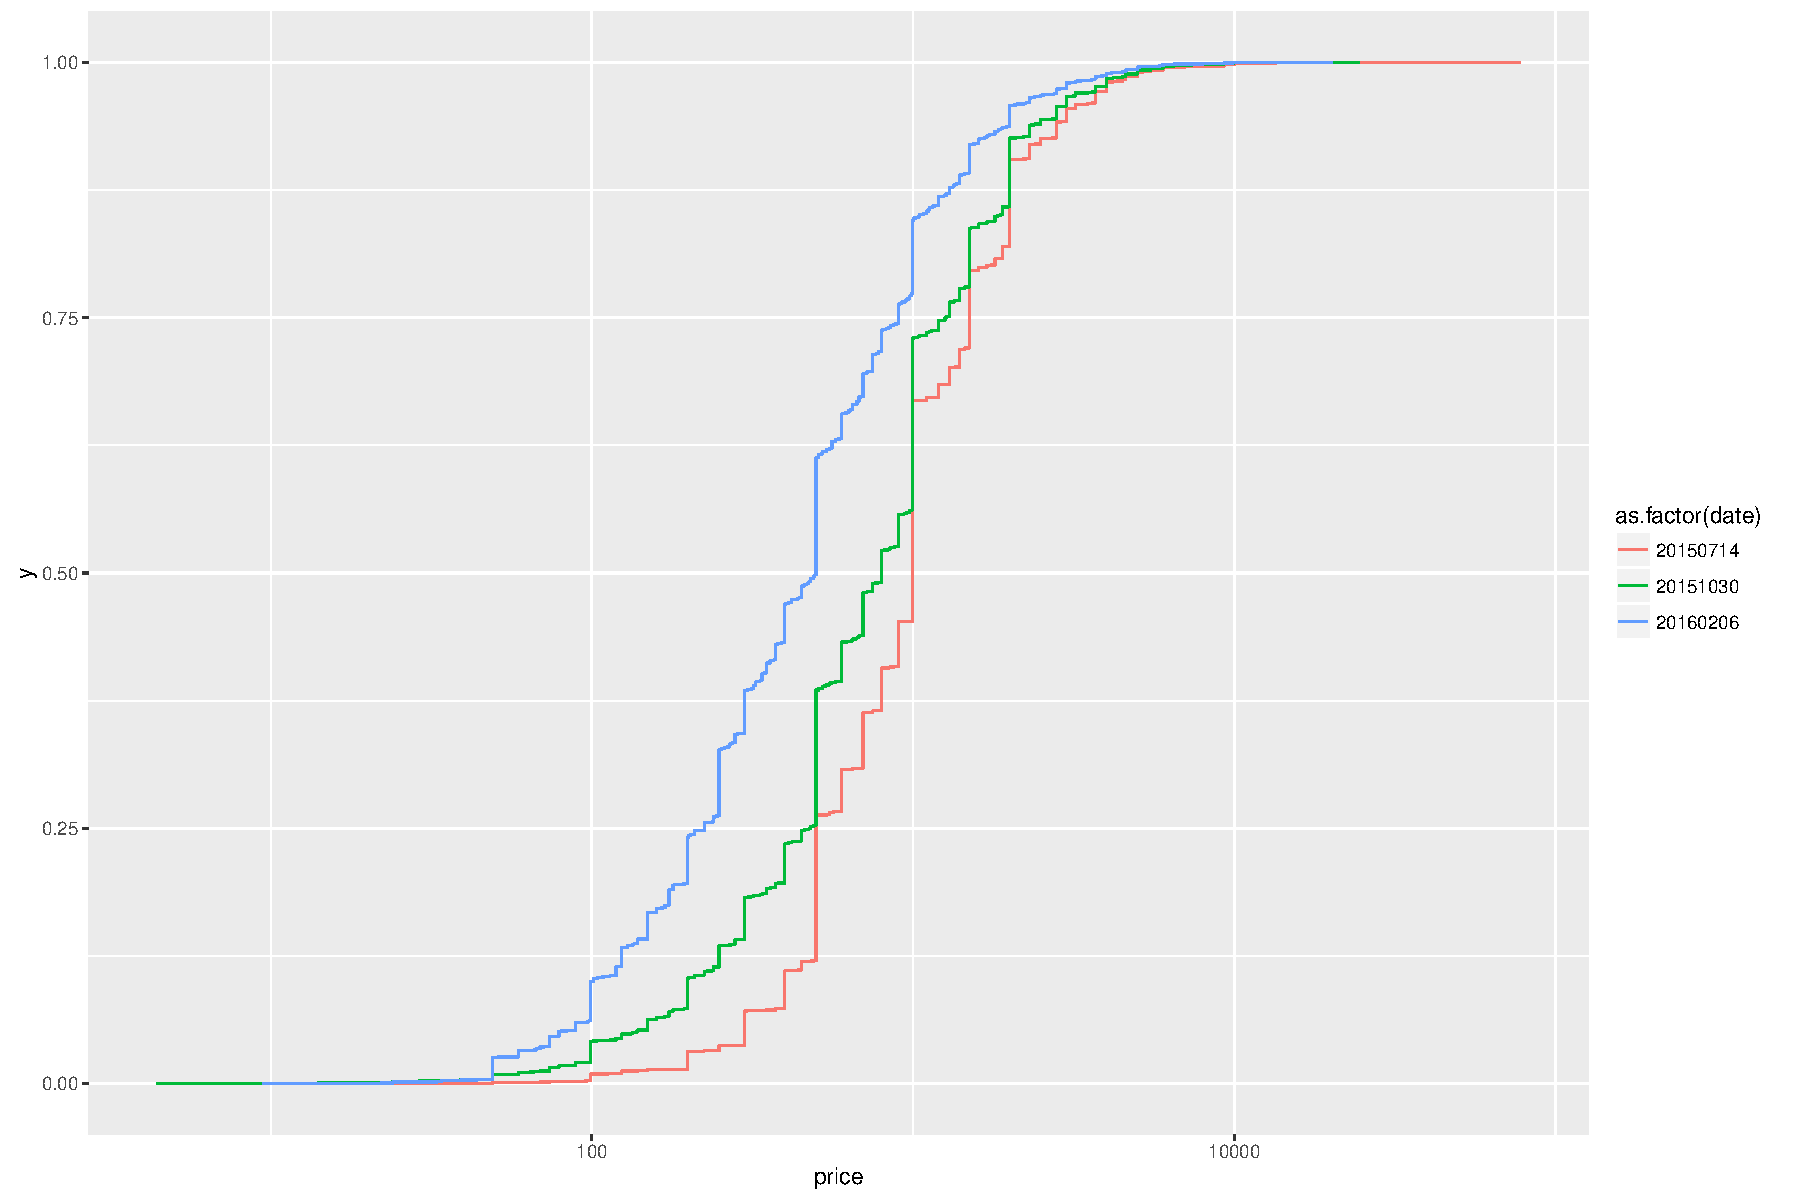
\includegraphics[width=1.0\columnwidth]{images/steam-prices.pdf}
	\caption{CDF of games on the steam platform at two distinct dates.}
\label{fig:steam-prices}
\end{figure}

Violinenplot der durchschnittlichen Spielzeit aufgeteilt auf unterschiedliche Preiskategorien. \ref{fig:steam-cost-vs-playtime-violin}

\begin{figure}[!t]
	\centering
	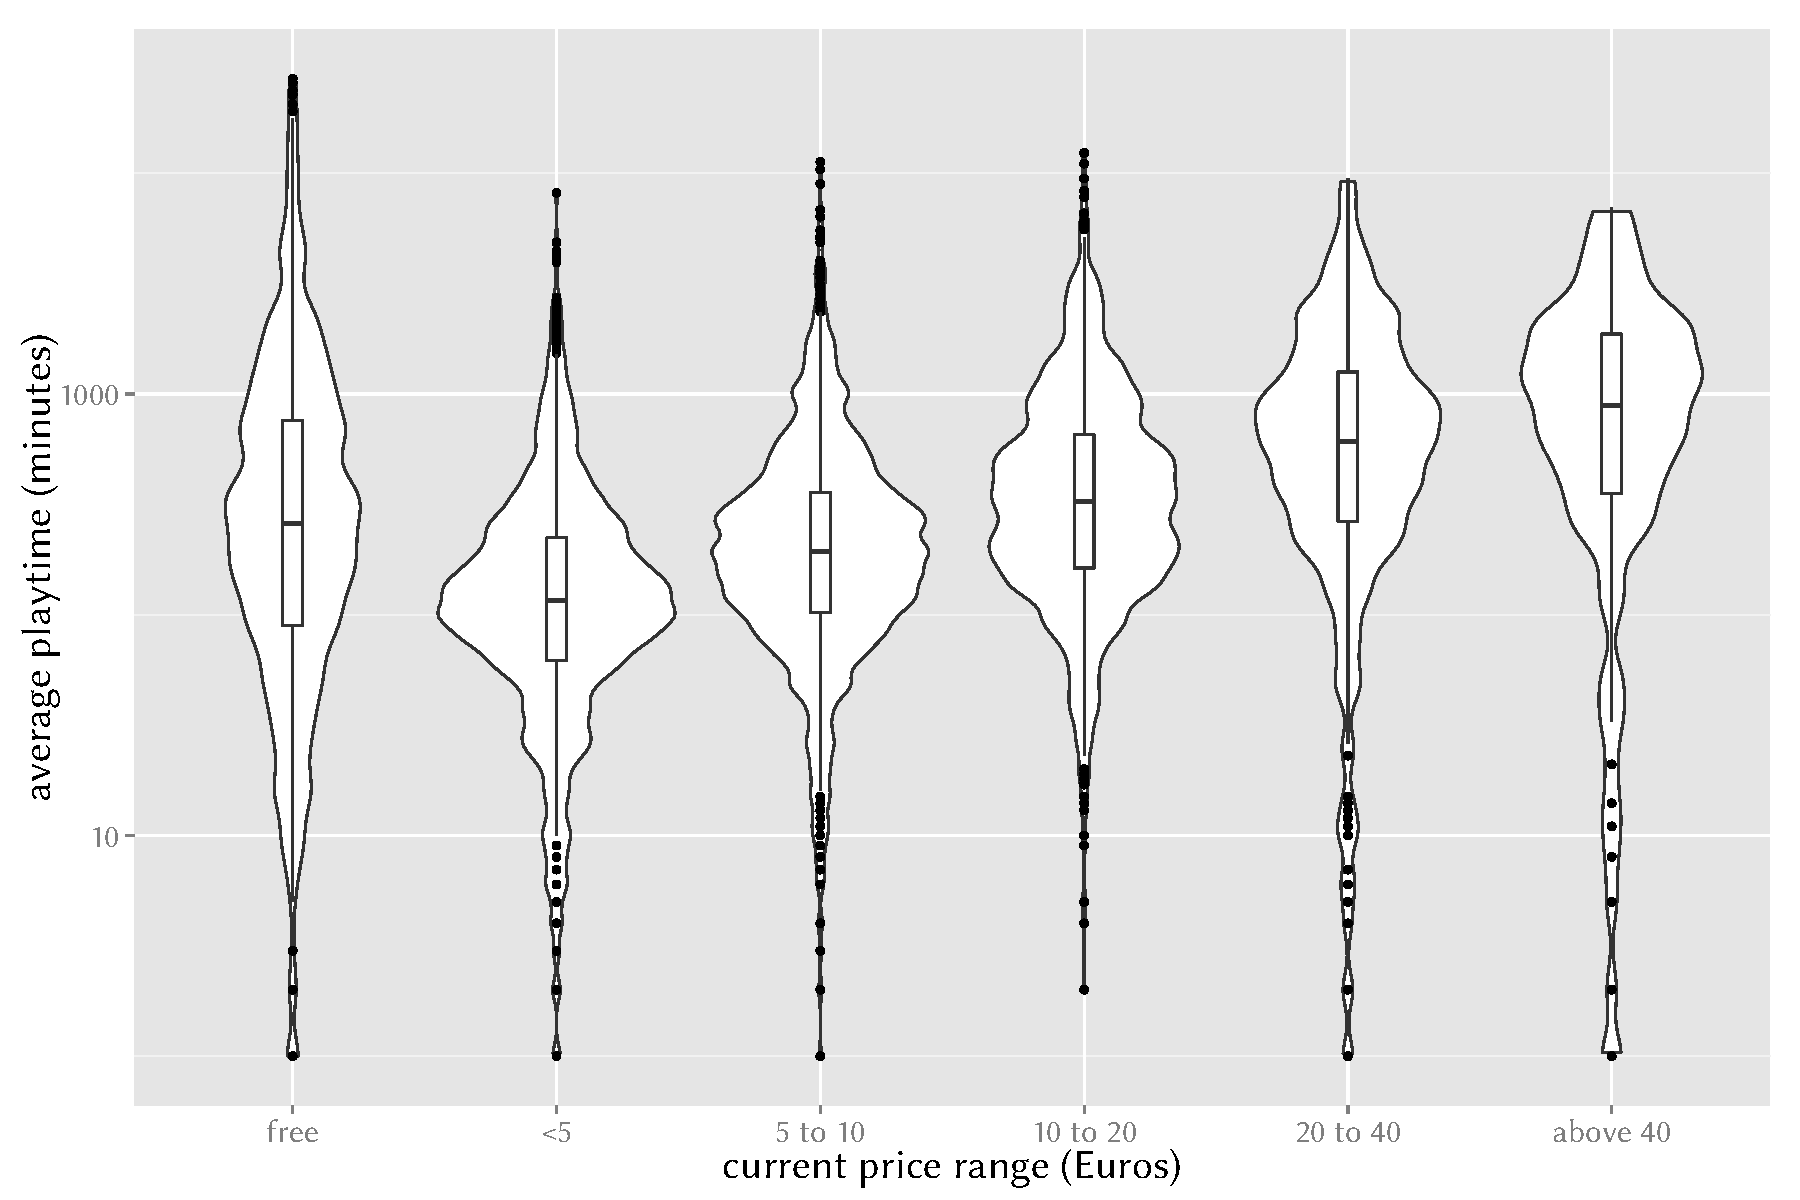
\includegraphics[width=1.0\columnwidth]{images/steam-cost-vs-playtime.pdf}
	\caption{Violin plot of the average playtime (as recorded by SteamSpy) of games categorized by their prices.}
\label{fig:steam-cost-vs-playtime-violin}
\end{figure}

%%%%%%%%%%%%
\subsubsection{HowLongToBeat Data}

Data scraped from \url{howlongtobeat.com}. This site allows for manual reporting of playthrough times of games on any platform. Times are separated into different play styles (e.g. ``main story'', ``completionist'') and only an aggregated time is shown. For this analysis only the average playtime of all play styles is taken into account.
It should however be stressed again, that this is a self-reporting site without strong validity checks. This has to be considered when contemplating the accuracy and validity of the data.

\begin{figure}[!t]
	\centering
	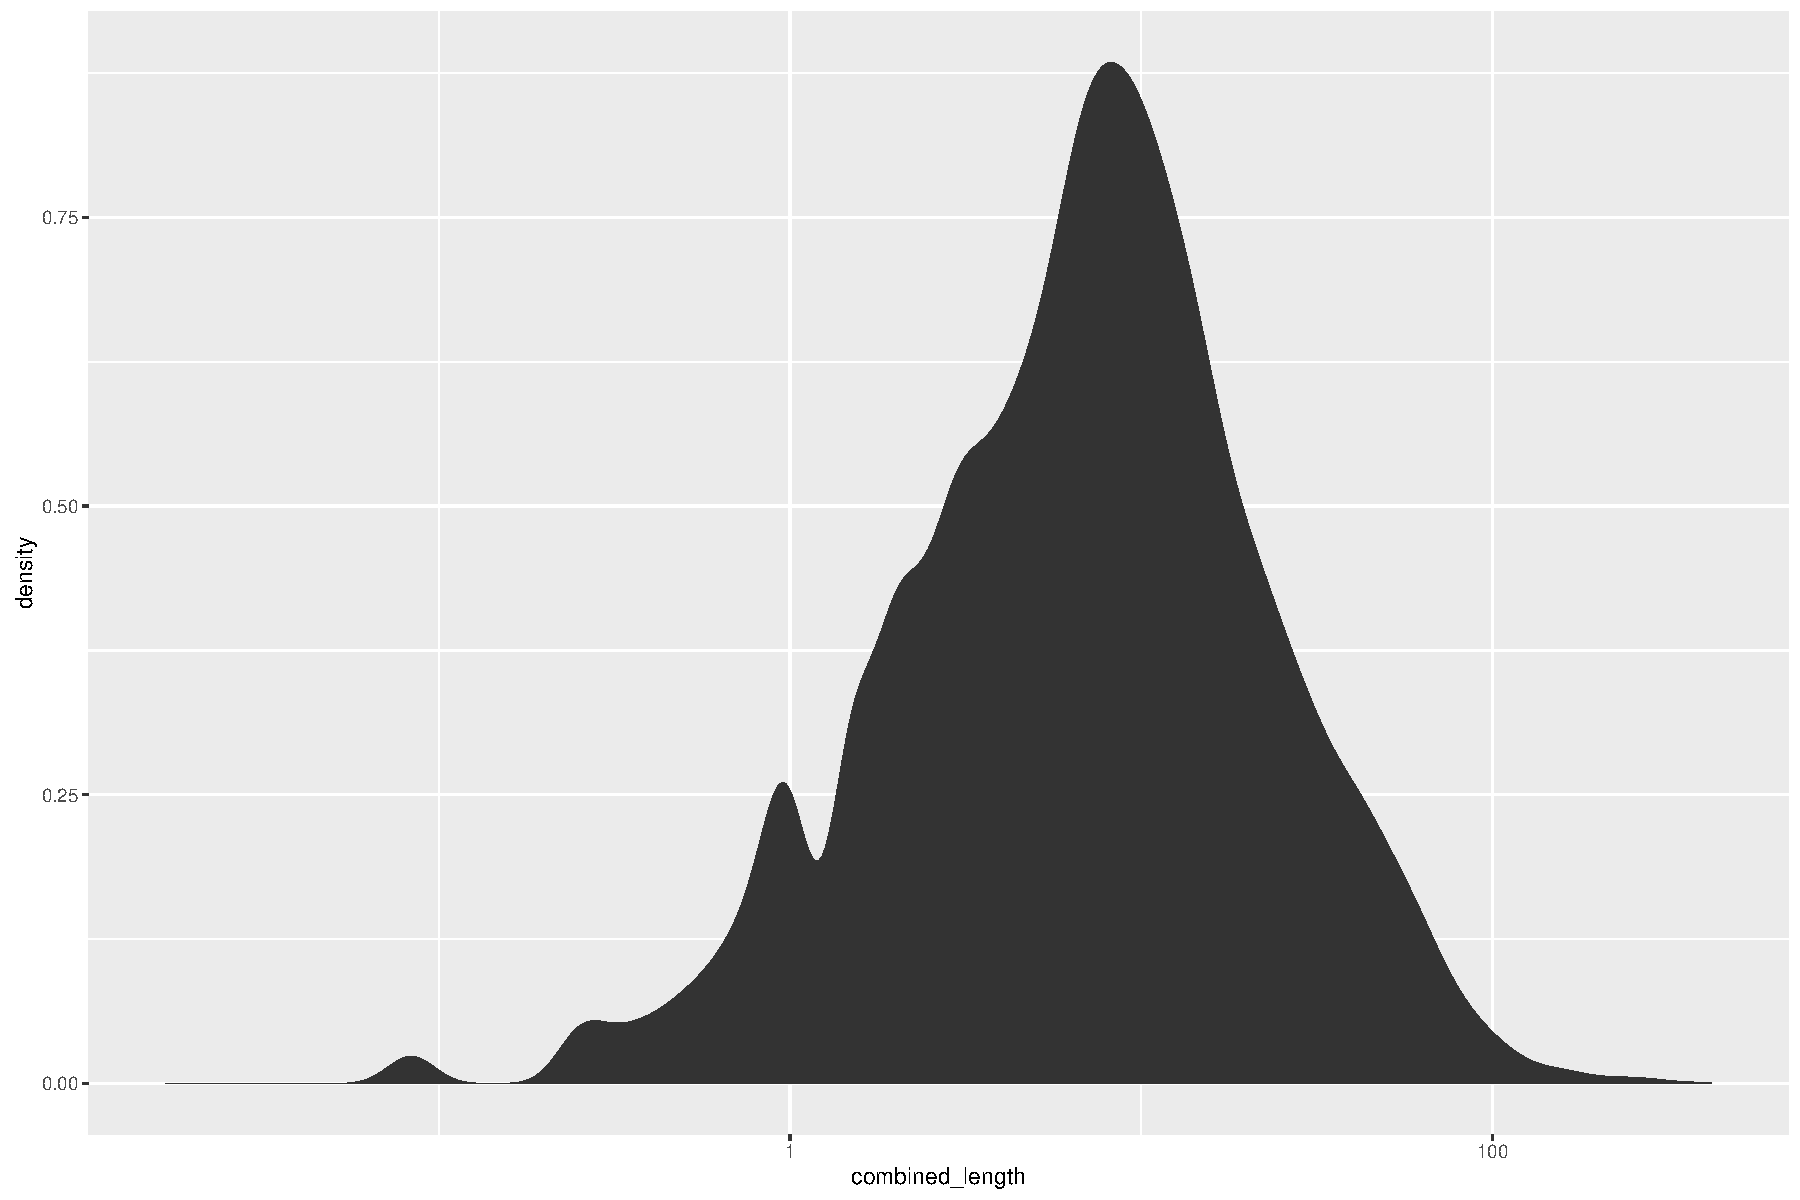
\includegraphics[width=1.0\columnwidth]{images/gamelengths-density.pdf}
	\caption{Density plot of the average game lengths over all play styles.}
\label{fig:gamelengths-density}
\end{figure}

Nonetheless, the distribution of game lengths from this set can still be worth to look at in the context of putting value to games for consumers of different platforms. As seen in Figure~\ref{fig:gamelengths-density} the play lengths vary greatly, with the median at \SI{7.5}{\hour} and a long tail of long play times reaching \SI{420}{\hour}.


%%%%%%%%%%%%
\subsubsection{Metacritic Data}

Game lengths can not only serve as an indicator of the amount of content a game has to offer, but can also serve as an engagement metric to estimate a user's amount of satisfaction. More fitting engagement metrics could also be employed.

% TODO: include or compare with data from opencritic.com as soon as their API is public/usable

\begin{figure}[!t]
	\centering
	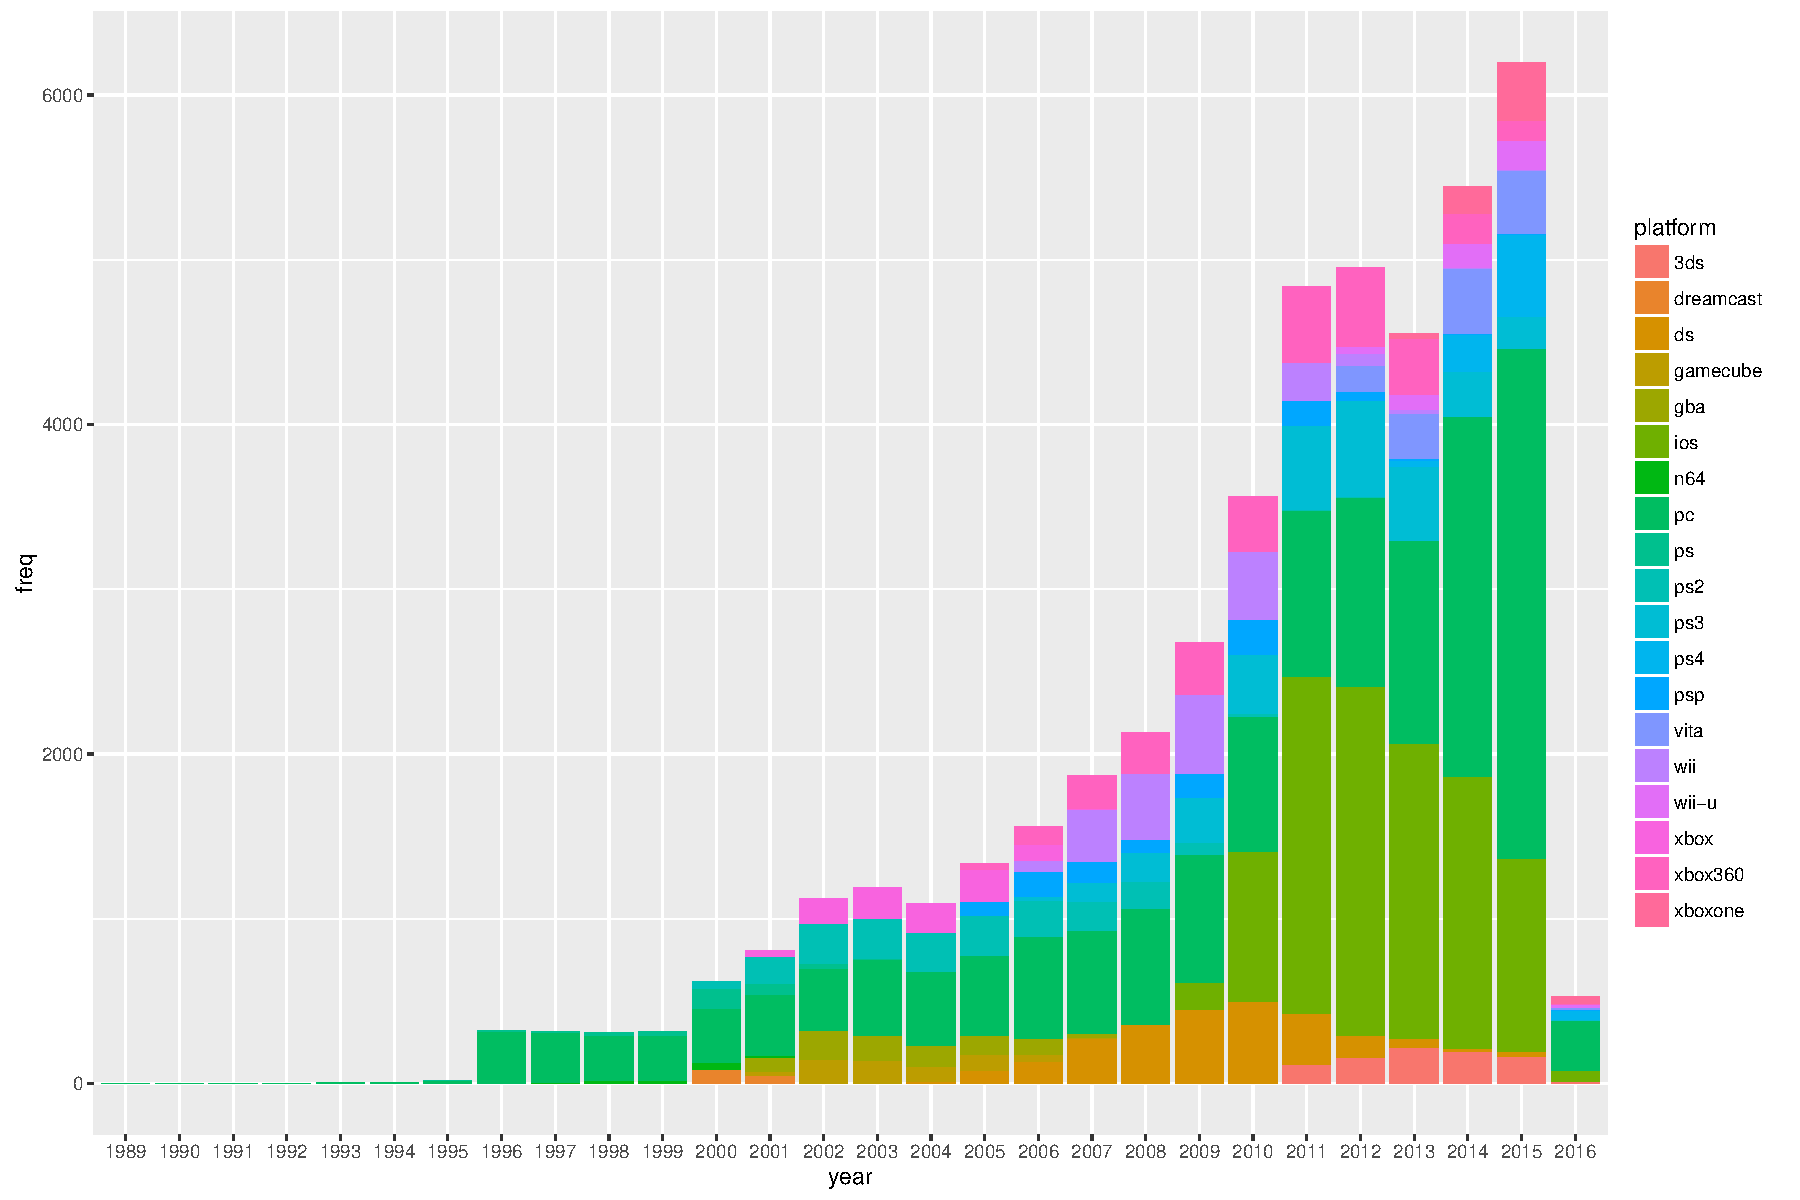
\includegraphics[width=1.0\columnwidth]{images/releases-per-year.pdf}
	\caption{Number of game releases per platform according to the Metacritic data.}
\label{fig:releases-per-year}
\end{figure}



%%%%%%%%%%%%
\subsubsection{platform-market-comparison/games-per-year.R}

 hat den ersten Versuch einer Nutzenrechnung für Spieler auf verschiedenen Plattformen. Script könnte leicht angepasst und erweitert werden. Beispielausgabe \ref{fig:gamesperyear-over-budget}, \ref{fig:steam-prices}

\begin{figure}[!t]
	\centering
	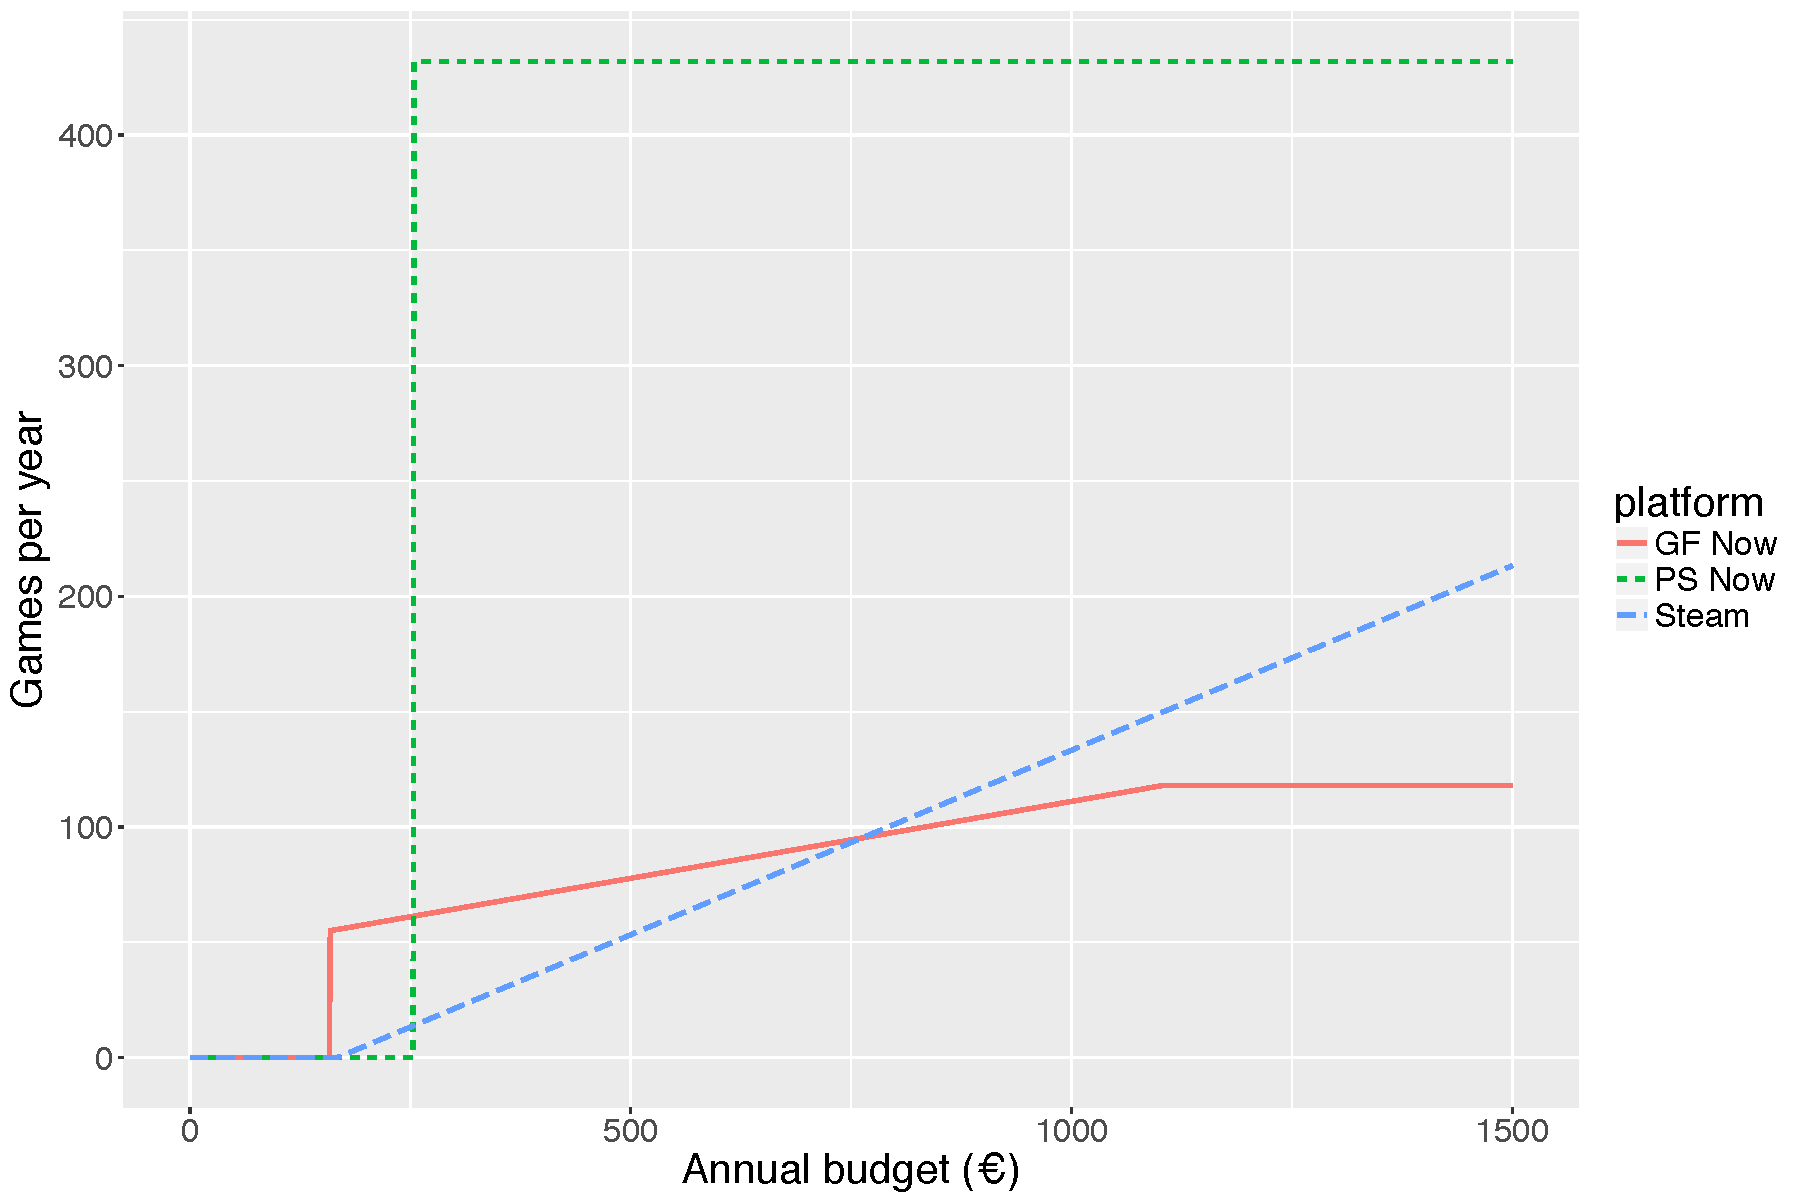
\includegraphics[width=1.0\columnwidth]{images/gamesperyear-over-budget.pdf}
	\caption{Models for several platforms showing the number of games per year that can be bought with a specific \$ budget.}
\label{fig:gamesperyear-over-budget}
\end{figure}

\begin{figure}[!t]
	\centering
	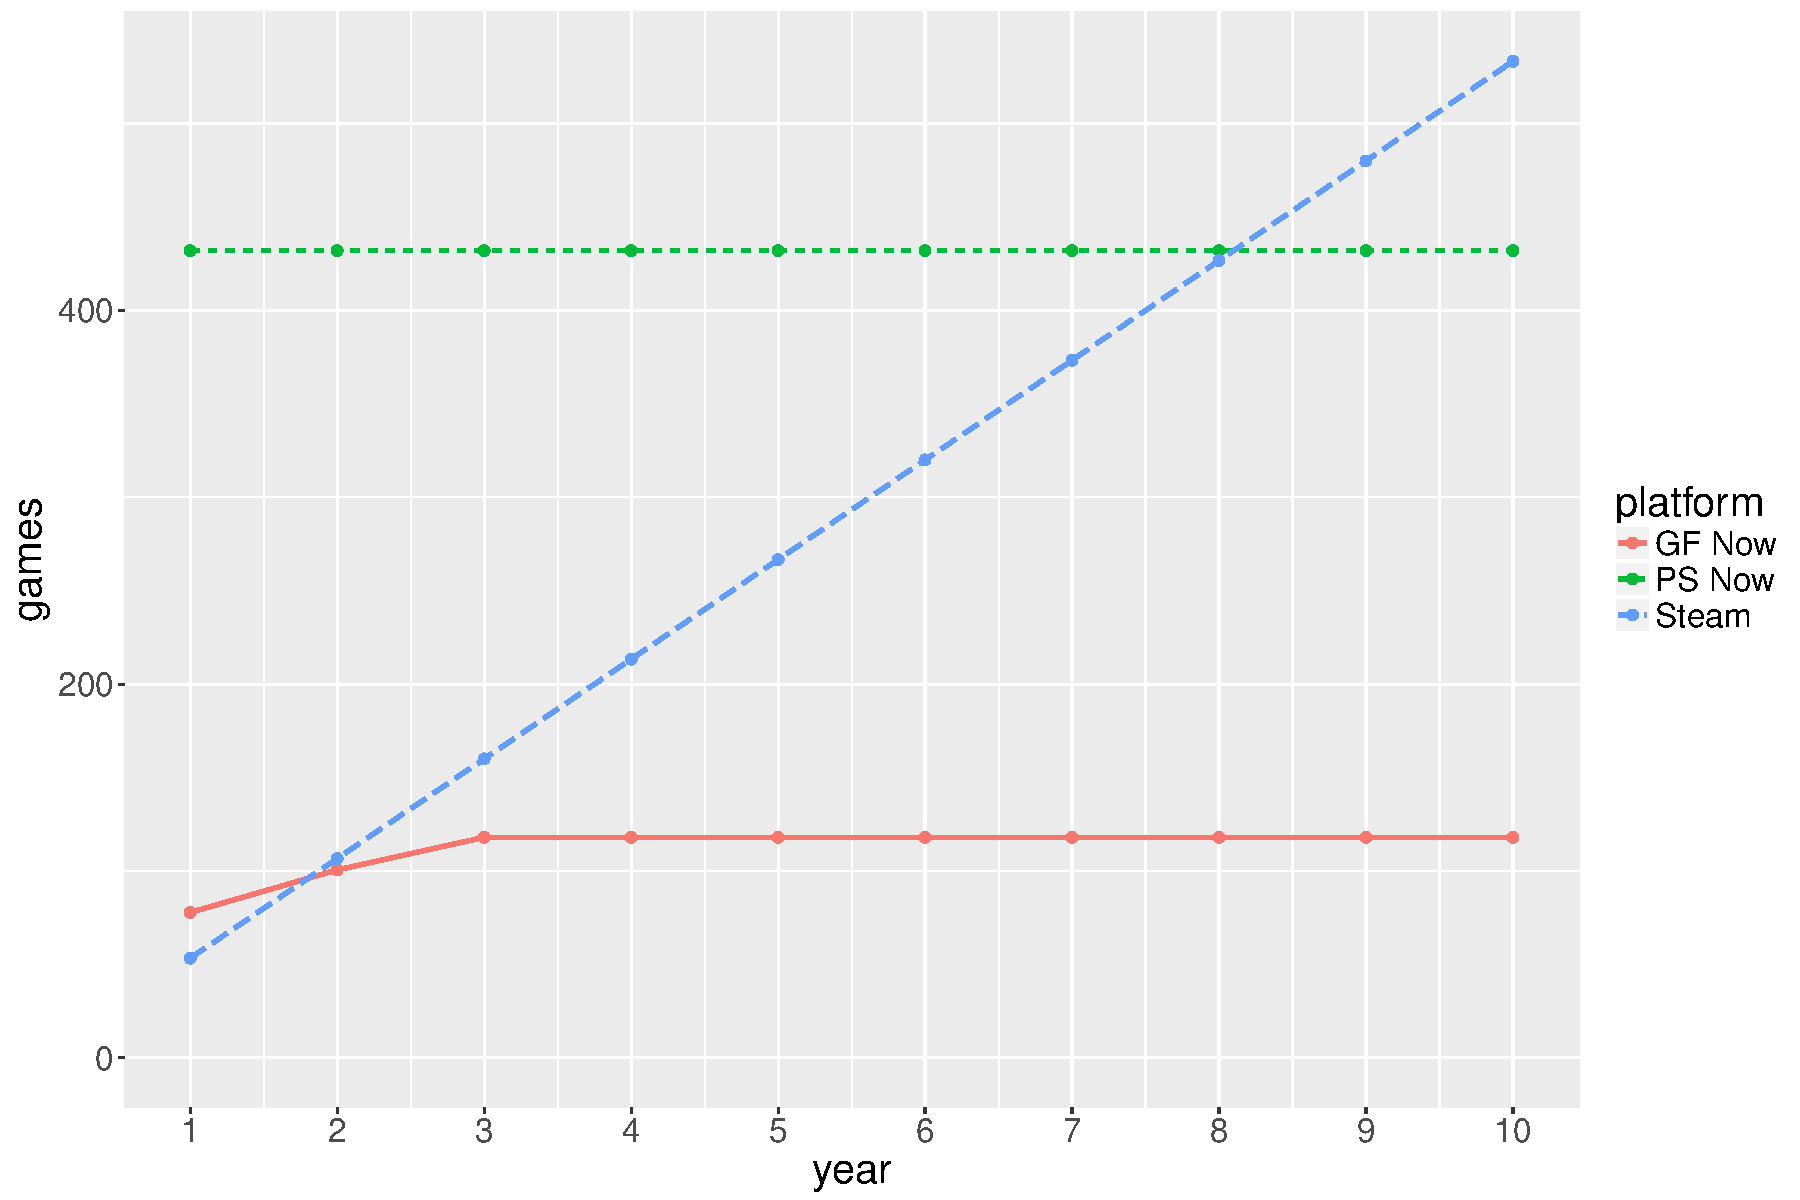
\includegraphics[width=1.0\columnwidth]{images/games-over-year.pdf}
	\caption{Models for several platforms showing the number of games that can be bought over the years subscribed to / using this service.}
\label{fig:games-over-years}
\end{figure}


\subsubsection{E2E Lag}
End-to-End Lag Model and Simulation in R. Now a standalone (submitted) paper at \url{https://github.com/mas-ude/onlinegame-lag-sim}. Can be referenced to argue the need for low E2E lag (meaning low network delay, but also the need for high fps).


%%%%%%%%%%%%
\subsubsection{Other Useful Data for Model Creation}

\begin{itemize}
	\item Game costs (current cost possible via Steam dataset; historic price data more difficult)
	\item Length of games (either via howlongtobeat dataset (via \url{https://github.com/mas-ude/gamelengths-scraper}), SteamSpy data, or could also additionally manually parse more Steam data)
	\item Gaming score/ratings/rankings (via Metacritic dataset (via \url{https://github.com/mas-ude/metacritic_scraper}), or might want to additionally scrape steam user review scores)
	\item Other popularity measures? (e.g. steamspy owner data?)
	\item Influence of E2E lag on games? (could be theorized indirectly through e2e lag sim + categorization attempts)
	\item Hardware requirements of games?

	\item Price History? Maybe using steamdb.info?
\end{itemize}


%!TEX root = paper.tex
%%%%%%%%%%%%%%%%%%%%%%%%%%%%%%%%%%%%%%%%%%%%%%%%%%%%%%%%%%%%%%%%%%%%%%%%%%%%%%%
\section{User Perspective and Prospects}
\label{sec:engagement}

To get a grasp of the value of the introduced platforms, this section examines the users' perspective by discussing applicable engagement metrics and by employing temporal cost-benefit models for hypothetical platform customers.

 %of gaming services, following a two-pronged approach. The first part introduces and discusses possible engagement metrics applicable to such services, while the second portion assembles some temporal cost-benefit models for hypothetical platform customers.


%%%%%%%%%%%%%%%%%%%%%%%%%%%%%%%%%%%%%%%%%%%%%%%%%%%%%%%%%%%%%%%%%%%%%%%%%%%%%%%%
\subsection{Engagement Metrics}

Metrics for user engagement, defined as ``\textit{the quality of the user experience that emphasises the positive aspects of the interaction, and in particular the phenomena associated with being captivated by a web application, and so being motivated to use it}''\cite{Lehmann2012}, can be used to compare different services against each other. The problem with engagement is finding the right measures befitting the type of service under scrutiny, in this case gaming, and cloud gaming in particular.

\begin{table*}
\centering
\caption{Overview of some simple engagement metrics comparing the three investigated services. Length data from \hltb, review scores from \metacritic.}
\label{tab:basic-engagement}
	\begin{tabu}{X[2]|X[r]X[r]X[r]X[r]X[r]X[r]X[r]X[r]X[r]}
	\toprule
	Service & Titles & Age $\mu$ & Age $\sigma$ & Length $\mu$ & Length $\sigma$ & Score $\mu$ & Score $\sigma$ & User Score $\mu$ & User Score $\sigma$\\
	\midrule
	\gfnow & $68$ & \SI{2.33}{\year} & \SI{1.95}{\year} & \SI{14.65}{\hour} & \SI{14.44}{\hour} & $75.9$ & $9.44$ & $72.41$ & $12.49$\\
	\psnow & $252$ & \SI{4.63}{\year} & \SI{2.5}{\year} & \SI{12.26}{\hour} & \SI{15.47}{\hour} & $76.72$ & $11.43$ & $73.1$ & $12.8$\\
	\steam & $7749$ & \SI{2.86}{\year} & \SI{3.96}{\year} & \SI{13.02}{\hour} & \SI{20.49}{\hour} & $71$ & $12$ & $69$ & $15.27$\\
	\bottomrule
	\end{tabu}
\end{table*}

So, which platform characteristics engage gamers? Compared to video content and video streaming platforms this is harder to answer due to the high diversity of both games and  gamers. Looking at some simple summary metrics in Tab.~\ref{tab:basic-engagement} does not give a clear picture, with one exception: the number of titles. The two relatively young cloud platforms offer a very limited number of games when compared to the games available on \steam, which itself again only represents a subset of all games available either solely on the PC (\metacritic lists $16192$) or across all platforms ($45803$ listed on the site). Due to the nature of the cloud services (streaming existing games) there are no ``platform exclusive'' titles, which often increases the attractiveness of a specific platform for specific audiences. These limits on variety might be one reason why \steam is much more compelling to wider audiences.
\footnote{PZ: Theoretically a game could be exclusive on a specific cloud service platform, which may not be good choice due to the small market, but theoretically it could work. Or not?}

The age of video games seems to be a relevant differentiator for a platform selection. Besides some memorable classics, customers may be most interested in most recent games due to technical quality improvements, social factors  and driven by advertisements and public appearances of the game. However, the average age of games is relatively high for the investigated cloud gaming platforms. While a similarly high value is observed for \steam, this is explained by the much wider range of offered games where despite the addition of new games older games are retained --- thus, the $\sigma$ for the game age is also higher. Additionally, \psnow might be a special case, as it is specifically advertised as a backwards compatibility for games that do not run on the latest Sony platform any more.% (the PlayStation 4 does not provide compatibility with its predecessors).

%Coupled with a higher $\sigma$ representing the wider range of games also in their age. 


 %The broad range of games available on \steam also increases the average age, seen here however 
 
\begin{figure}[!t]
	\centering
	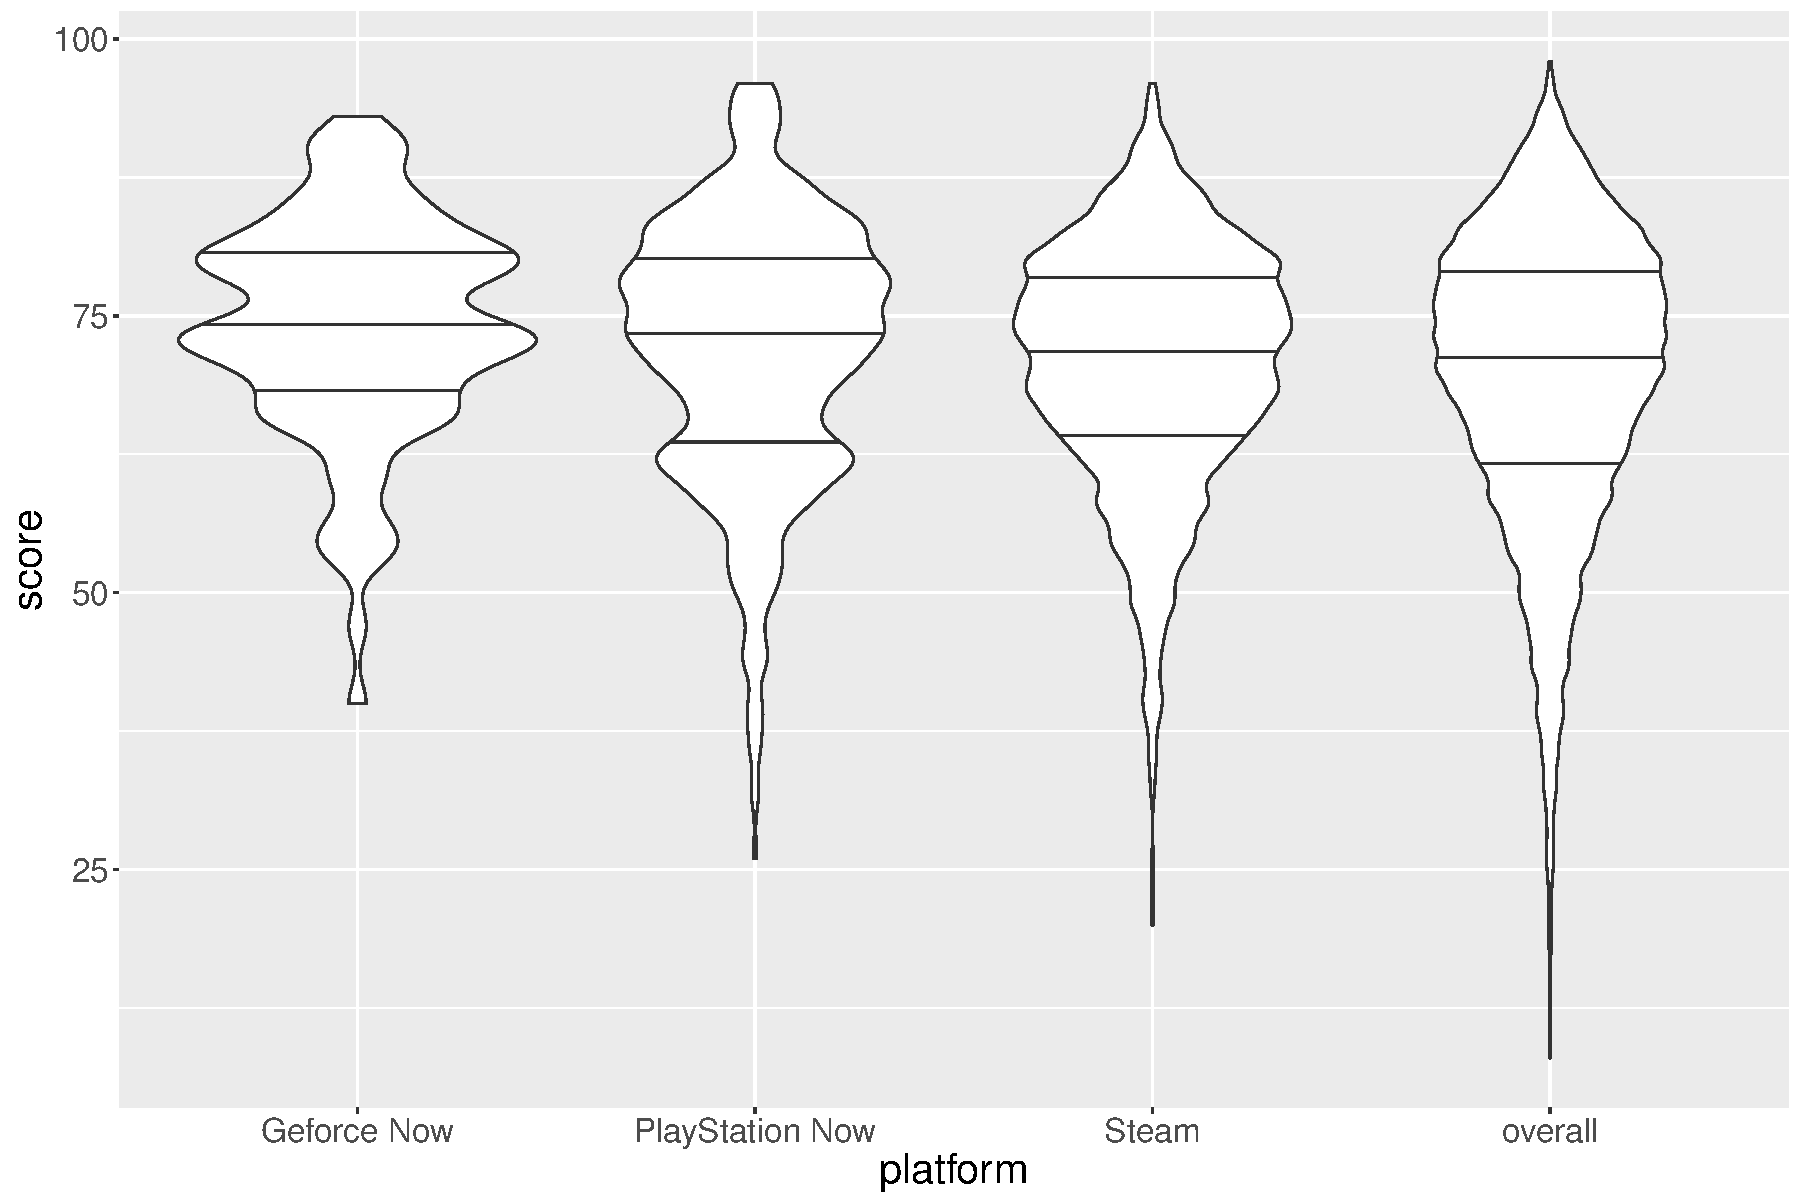
\includegraphics[width=1.0\columnwidth]{images/scores-by-platform-violin.pdf}
	\caption{Distribution of aggregated review scores per platform as violin plot with $25\%$, $50\%$ and $75\%$ quantiles.}
\label{fig:scores-by-platform}
\end{figure}

A third examined factor are the review scores as collected in the \metacritic set which seem quite similar across all services, albeit with a slightly lower $\sigma$ for \gfnow. This can probably be attributed to both the small scale and through manual curation. Though, the mean values do not expose the whole picture of review scores, as evident in the violin plots of Fig.~\ref{fig:scores-by-platform}. Both streaming services seem to favor certain score levels. Specifically, they both show a number of highly rated titles, followed by a bulge of average ratings and few but noticeable titles in the low score tail. These could be indications of the different nature of today's cloud gaming ecosystems. \steam on the one side is a more or less open platform, where every game publisher can sell their games at their own volition (platform operator collects a commission fee for sales). Cloud gaming platforms have to acquire licenses from the individual games' publishers and therefore have to be selective and curated by nature. 

A closer look at the \metacritic scores for assessing engagement reveals a small correlation between general score and number of game ownerships on \steam (as an indicator for popularity of a game): Pearson correlation coefficient $= 0.1998204$. Interestingly, for \metacritic user scores the effect turns out to be smaller (Pearson correlation $= 0.1010024$). 
\todo[inline]{PZ: And that tells us what?}

Finally, the length of games is an example of content-based engagement factors. To assume that a longer game might be more engaging to many players might be a viable assessment. But this would need further validation, as it does characterise the quality of the game. As a first indicator the correlation coefficient between number of game ownerships on \steam and combined game length from the \hltb dataset reveal a small effect (Pearson correlation $= 0.175819$, see figure \ref{fig:rel-combinedlength-owners}). Again, all three platforms are rather closely grouped together in this metric, with the one exception being \steam's variance being higher, signifying once again a broader range of available game titles.



\begin{figure}[!t]
	\centering
	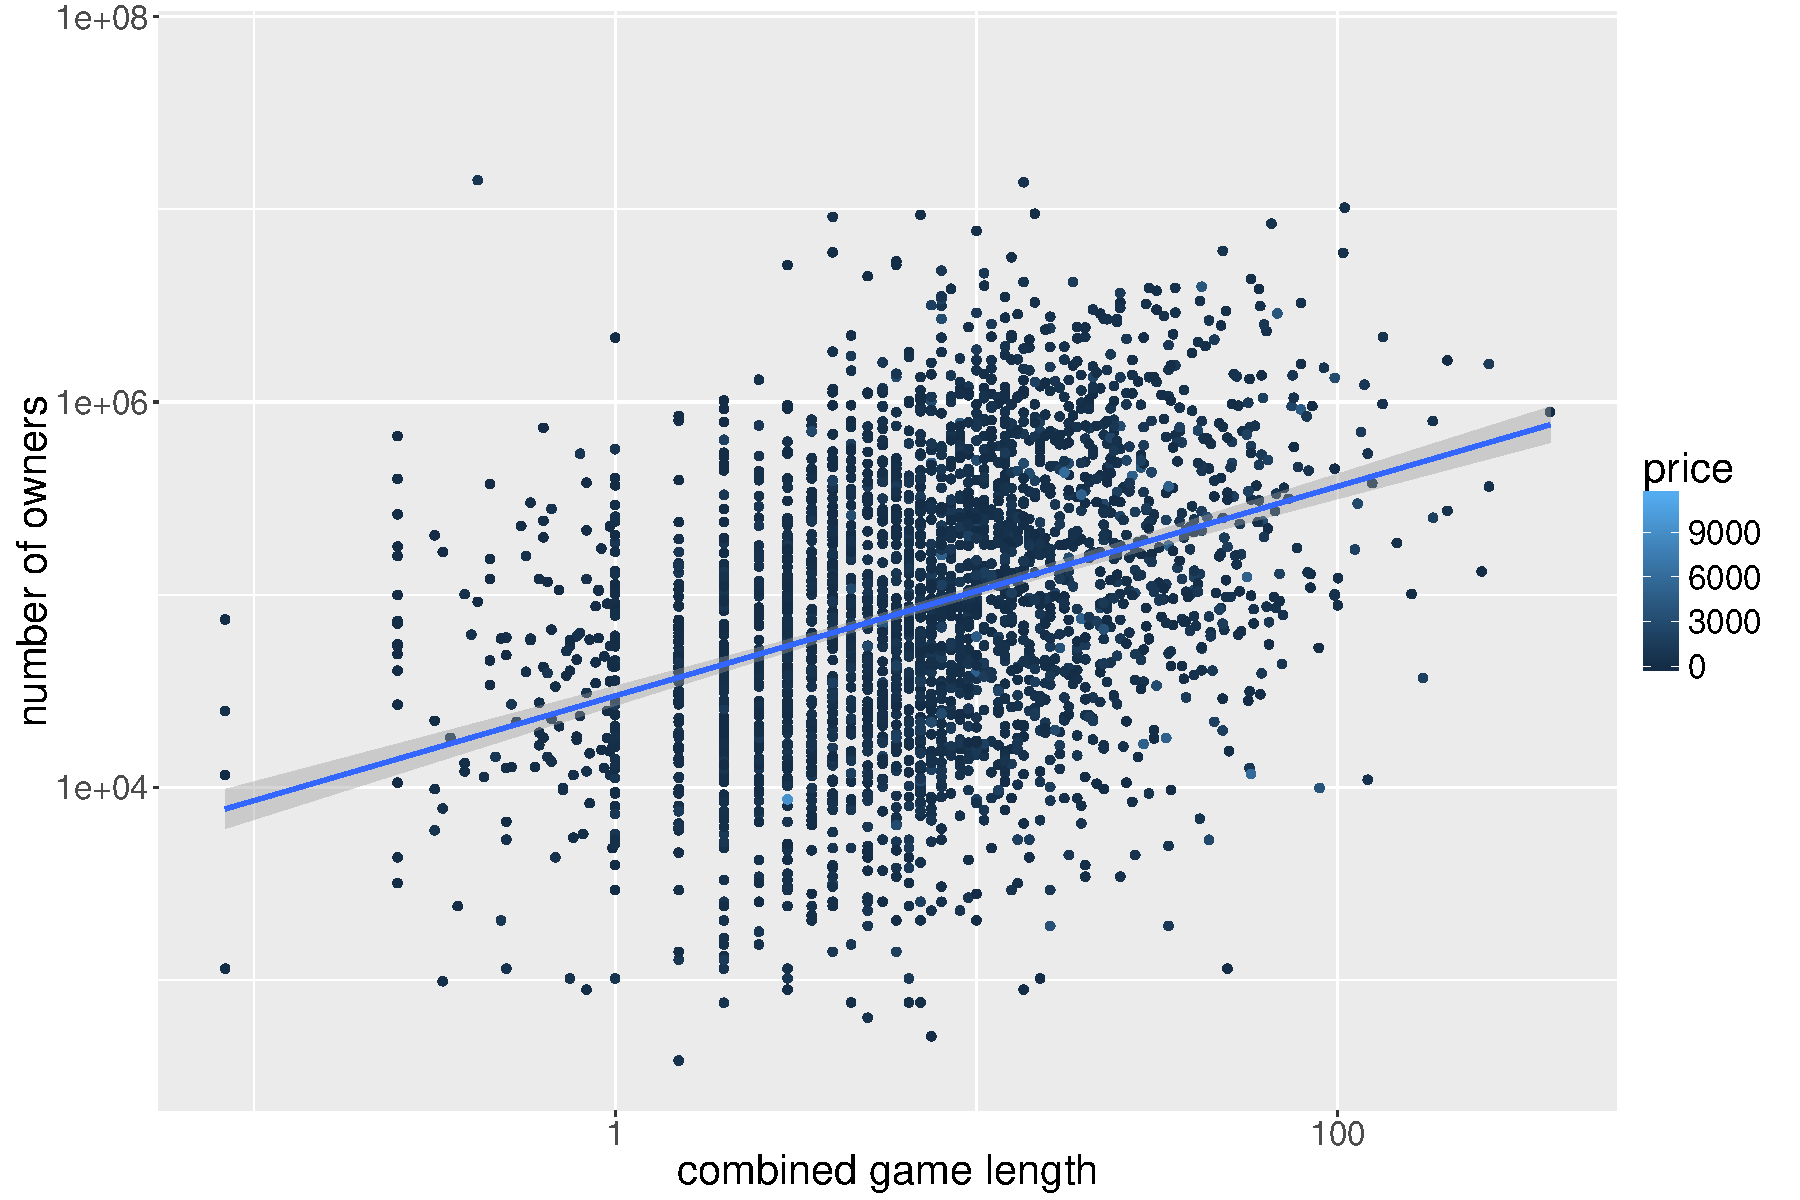
\includegraphics[width=1.0\columnwidth]{images/rel-combinedlength-owners.pdf}
	\caption{Relationship game length to ownership}
\label{fig:rel-combinedlength-owners}
\end{figure}


%%%%%%%%%%%%
\subsubsection{Further Potential Engagement Factors}

Due to the limited amount of available data the number of currently observable potential engagement metrics is restricted. However, many more come to mind and are worth investigating in the future. These could include,

\begin{itemize}
	\item the number of platform ``exclusive'' game titles,
	\item the genre as well as other classifications of games,
	\item the number of game sales and subscriber numbers,
	\item more objective measures of the game's content (e.g. the variety and quality of game mechanics),
	\item technical aspects of games (e.g. the graphical fidelity, the performance, or the precision and responsiveness of controls),
	\item or other content-centric factors based on the games' content.
\end{itemize}




%However, when having a look at figures \ref{fig:rel-price-category-owners} and \ref{fig:rel-score-category-owners}, 
%Some details remain unclear: Despite having a relatively low Metacritic score, especially games within the 11-20 range seem to have quite a number of owners - why? Also, either games for free or expensive games seem to be popular. Maybe this is an indicator for the differentiation between hardcore and casual gamers? (Probably it would be interesting as well to track the price over the years and also weigh the ownership count relatively to a game's age.)

%\begin{figure}[!t]
%	\centering
%	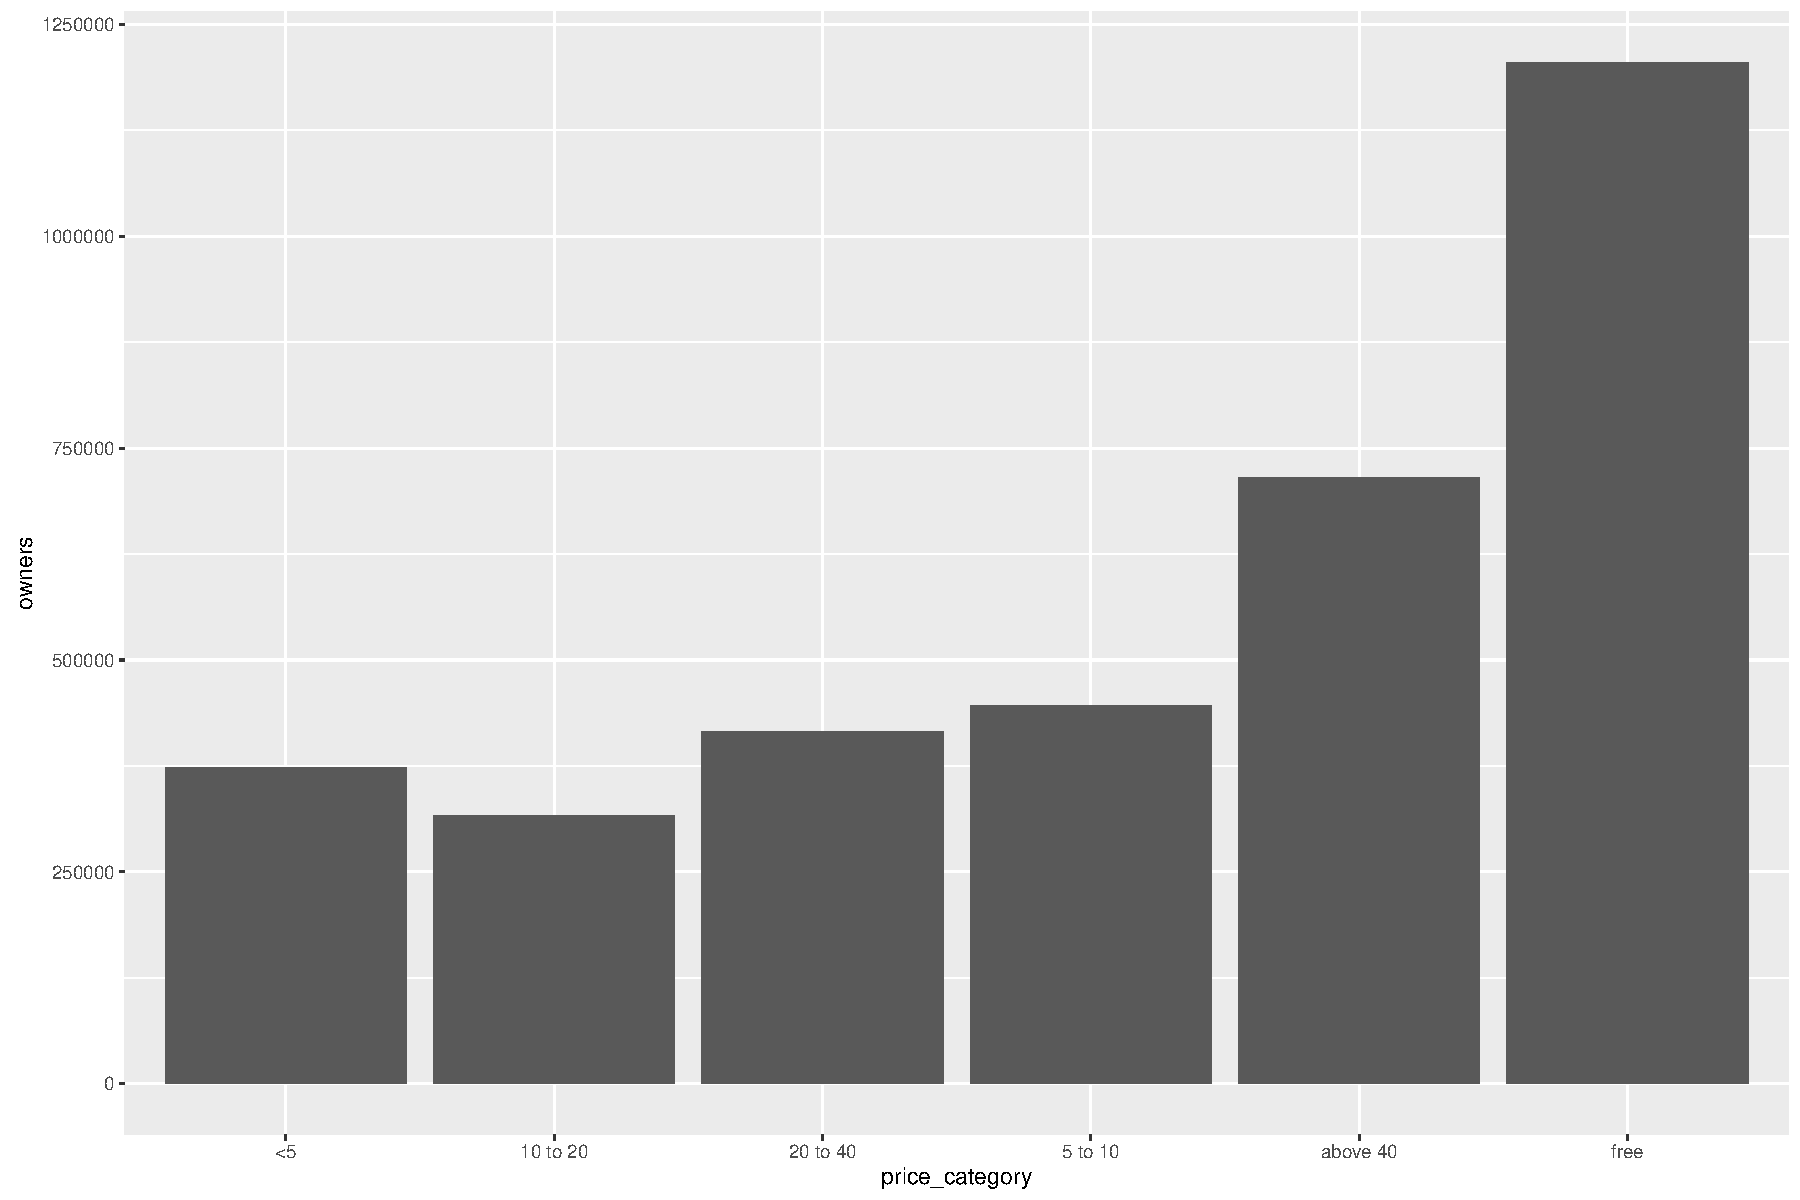
\includegraphics[width=1.0\columnwidth]{images/rel-price-category-owners.pdf}
%	\caption{Relationship price category to ownership (\textbf{TODO: Bars need sorting})}
%\label{fig:rel-price-category-owners}
%\end{figure}
%
%\begin{figure}[!t]
%	\centering
%	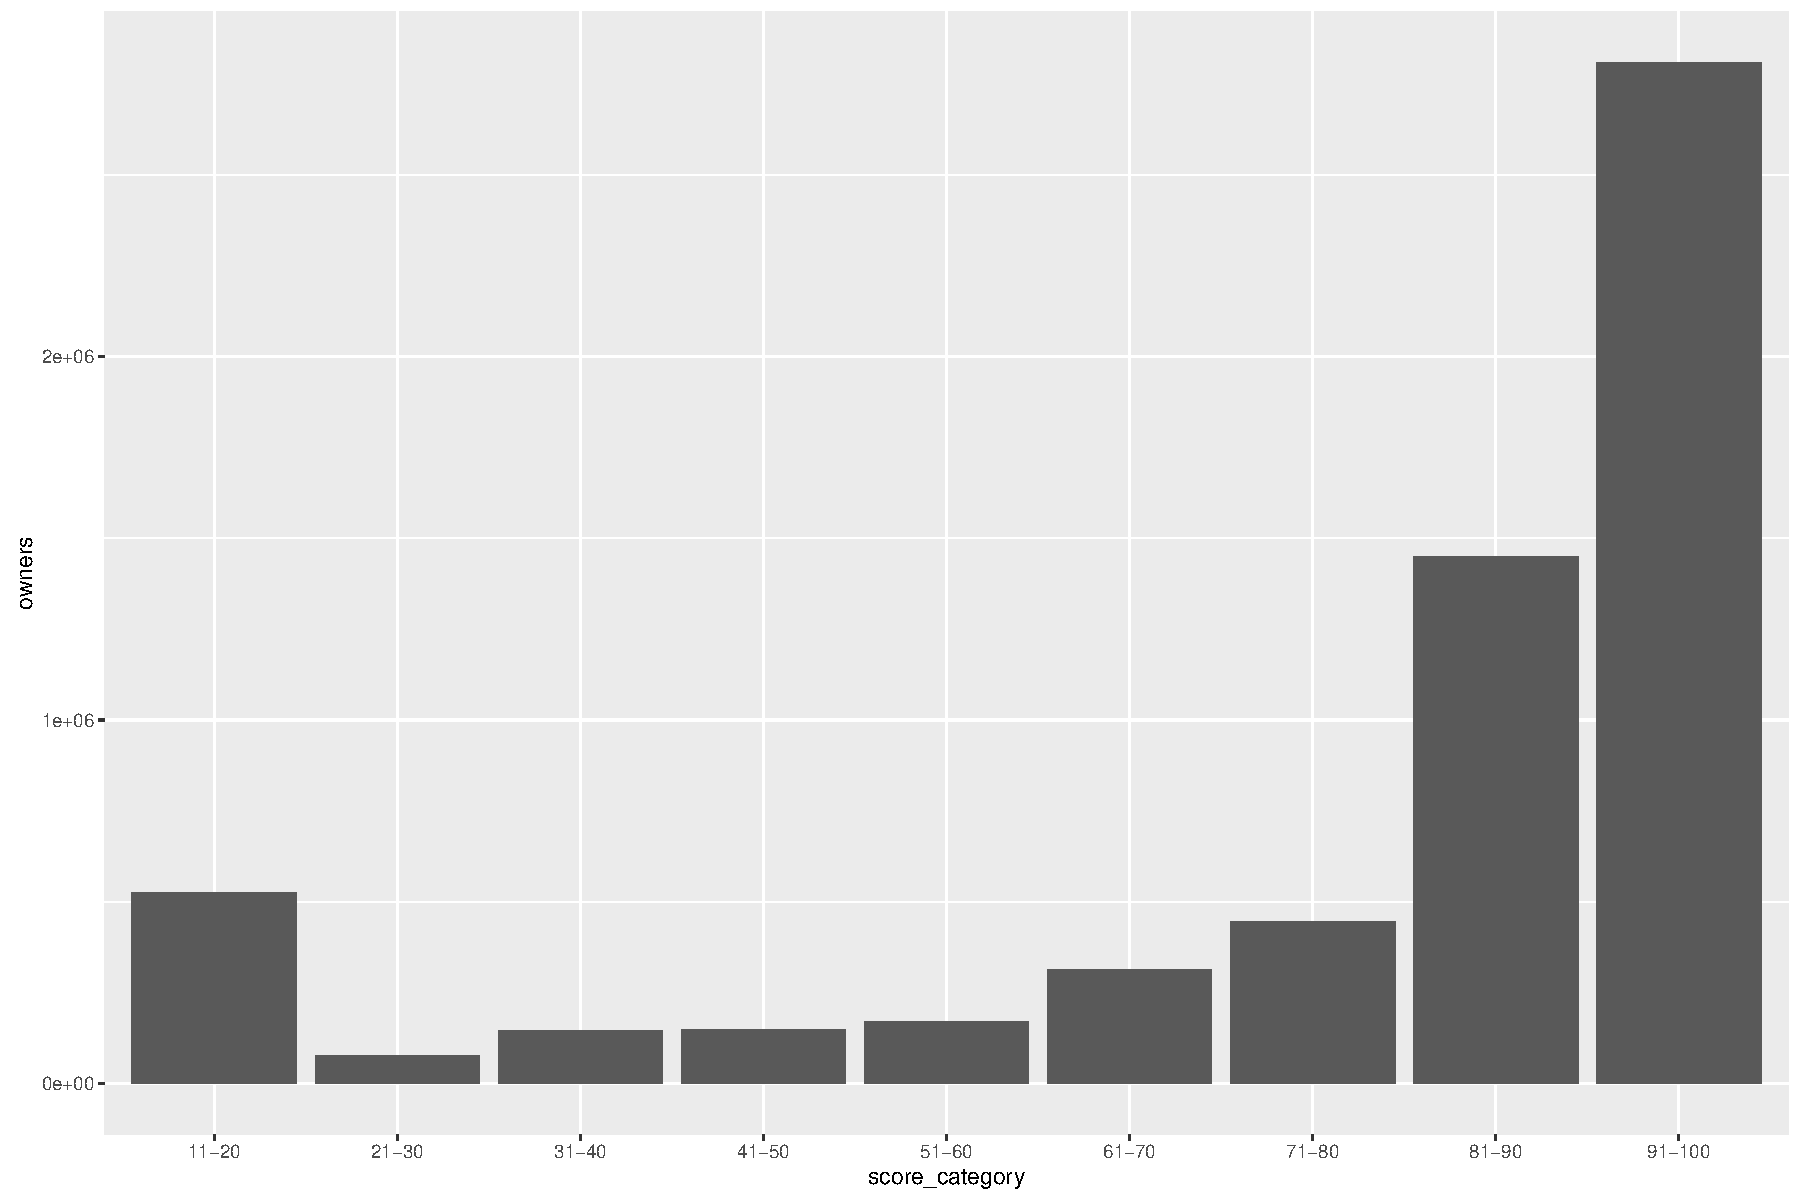
\includegraphics[width=1.0\columnwidth]{images/rel-score-category-owners.pdf}
%	\caption{Relationship score category to ownership (\textbf{TODO: Bars need sorting})}
%\label{fig:rel-score-category-owners}
%\end{figure}


%%%%%%%%%%%%%%%%%%%%%%%%%%%%%%%%%%%%%%%%%%%%%%%%%%%%%%%%%%%%%%%%%%%%%%%%%%%%%%%%
\subsection{Cost-Benefit Models}


The price models for cloud services, as deliberately excluded in the discussion of engagement metrics, largely differ from the approach of \steam. Setting the number of games, as noteworthy value metric, in relationship to the cost or budget (service price), two simple models are created. Naturally, this does not factor in any user preferences to specific games and their availability on just a subset of platforms. But the current curated nature of Cloud Gaming platforms would prevent this endeavour from succeeding regardless.

\todo[inline]{PZ: Which models? Or what are the models?}

%Moreover, the examined engagement metrics do not provide many means for a service distinction bar the number of games available. Therefore, the two simple models provided here use the number of affordable games on a specific budget. 

For both models a few basic assumptions are made. The initial hardware costs are factored in proportionately to the expected life and depreciation time of the devices, which is assumed to be \SI{3}{\year} for PCs and \SI{7}{\year} for the consoles and devices necessary to receive the streaming service (\SI{7}{\year} is about the average life cycle of a video game console generation and should be representative in this case).

What should also be noted is the difference in the service model between the ownership model of \steam, the hybrid subscription plus permanent rental model of \gfnow, as well as the subscription and timed rental model of \psnow. For the latter rentals subscription is also not a prerequisite. As this subtle differences are difficult to express in a simple cost-benefit model, they are all treated the same here. Therefore, they are all treated equally in the models as games, that one has access to and could have been played at one point. Other means of acquiring games cheaper from outside of the respective services, of which there are many for PC gaming as discussed in Sec.~\ref{sec:pcgaming}, are also omitted here.

%%%%%%%%%%%%%%%%%%%%%%%%%%%%%%%%%%%%%%%%%%%%%%
\paragraph{Affordable Games on a Budget Model}

The first model assumes that one has a fixed budget to spend on video games. This model then shows, depending on the size of the budget, how many games one would be able to afford considering all initial and continual costs.

\begin{figure}[!t]
	\centering
	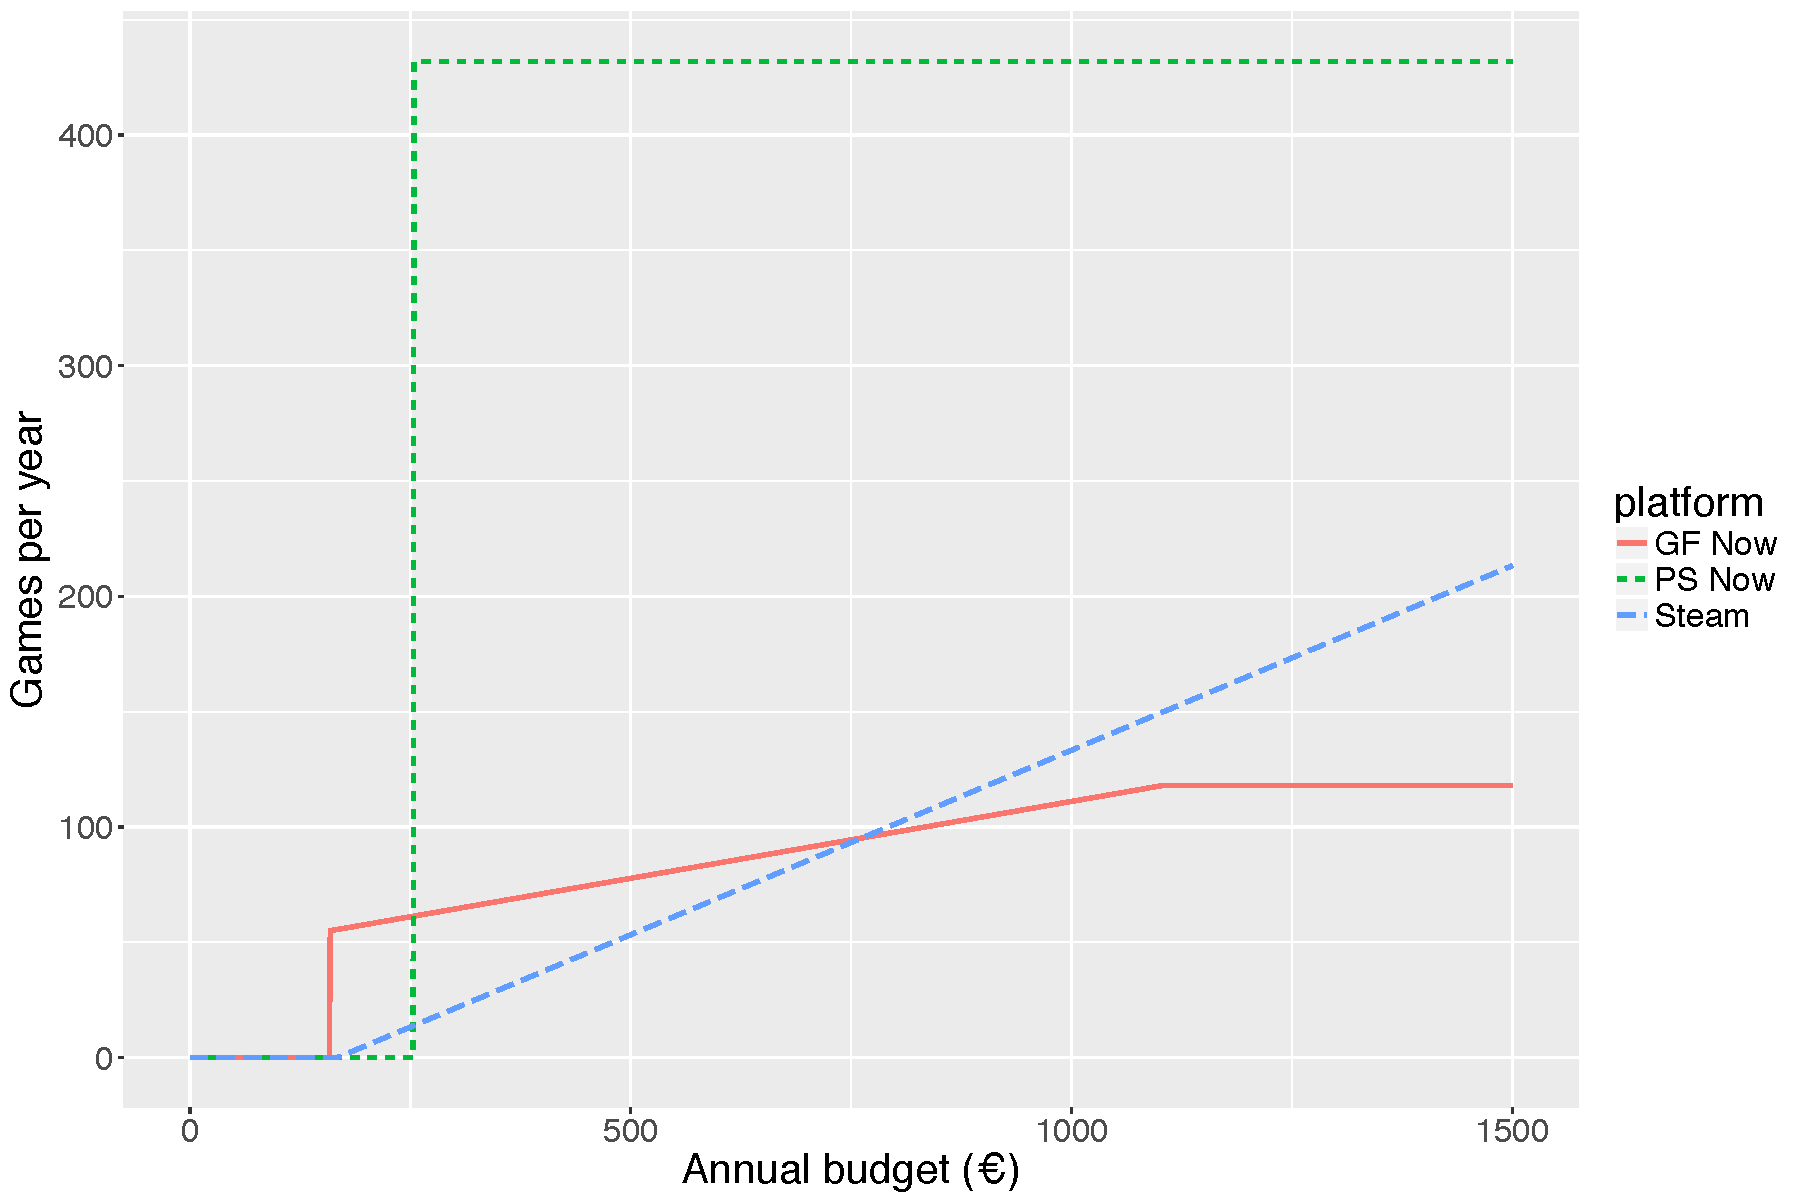
\includegraphics[width=1.0\columnwidth]{images/gamesperyear-over-budget.pdf}
	\caption{Per-platform price models as relationship of offered games (y-axis) in customer expenditure (budget; x-axis).}
\label{fig:gamesperyear-over-budget}
\end{figure}

As evident in Fig.~\ref{fig:gamesperyear-over-budget} all platforms start with relatively high fix costs, but only the subscription models provide instant access to a certain amount of titles, which could make them more attractive to newcomers on a low budget. Once one gets more interested in gaming and has access to a somewhat higher budget, the limited nature of both \psnow and \gfnow becomes evident.


%%%%%%%%%%%%%%%%%%%%%%%%%%%%%%%%%%%%%%%%%%%
\paragraph{Affordable Games per Year Model}

The second model extends the previous budget model to a longer time period of several years, investigating the value one gets if only a very low annual budget is spent. For the exemplary model it is assumed to be \SI{500}{\EUR}

\begin{figure}[!t]
	\centering
	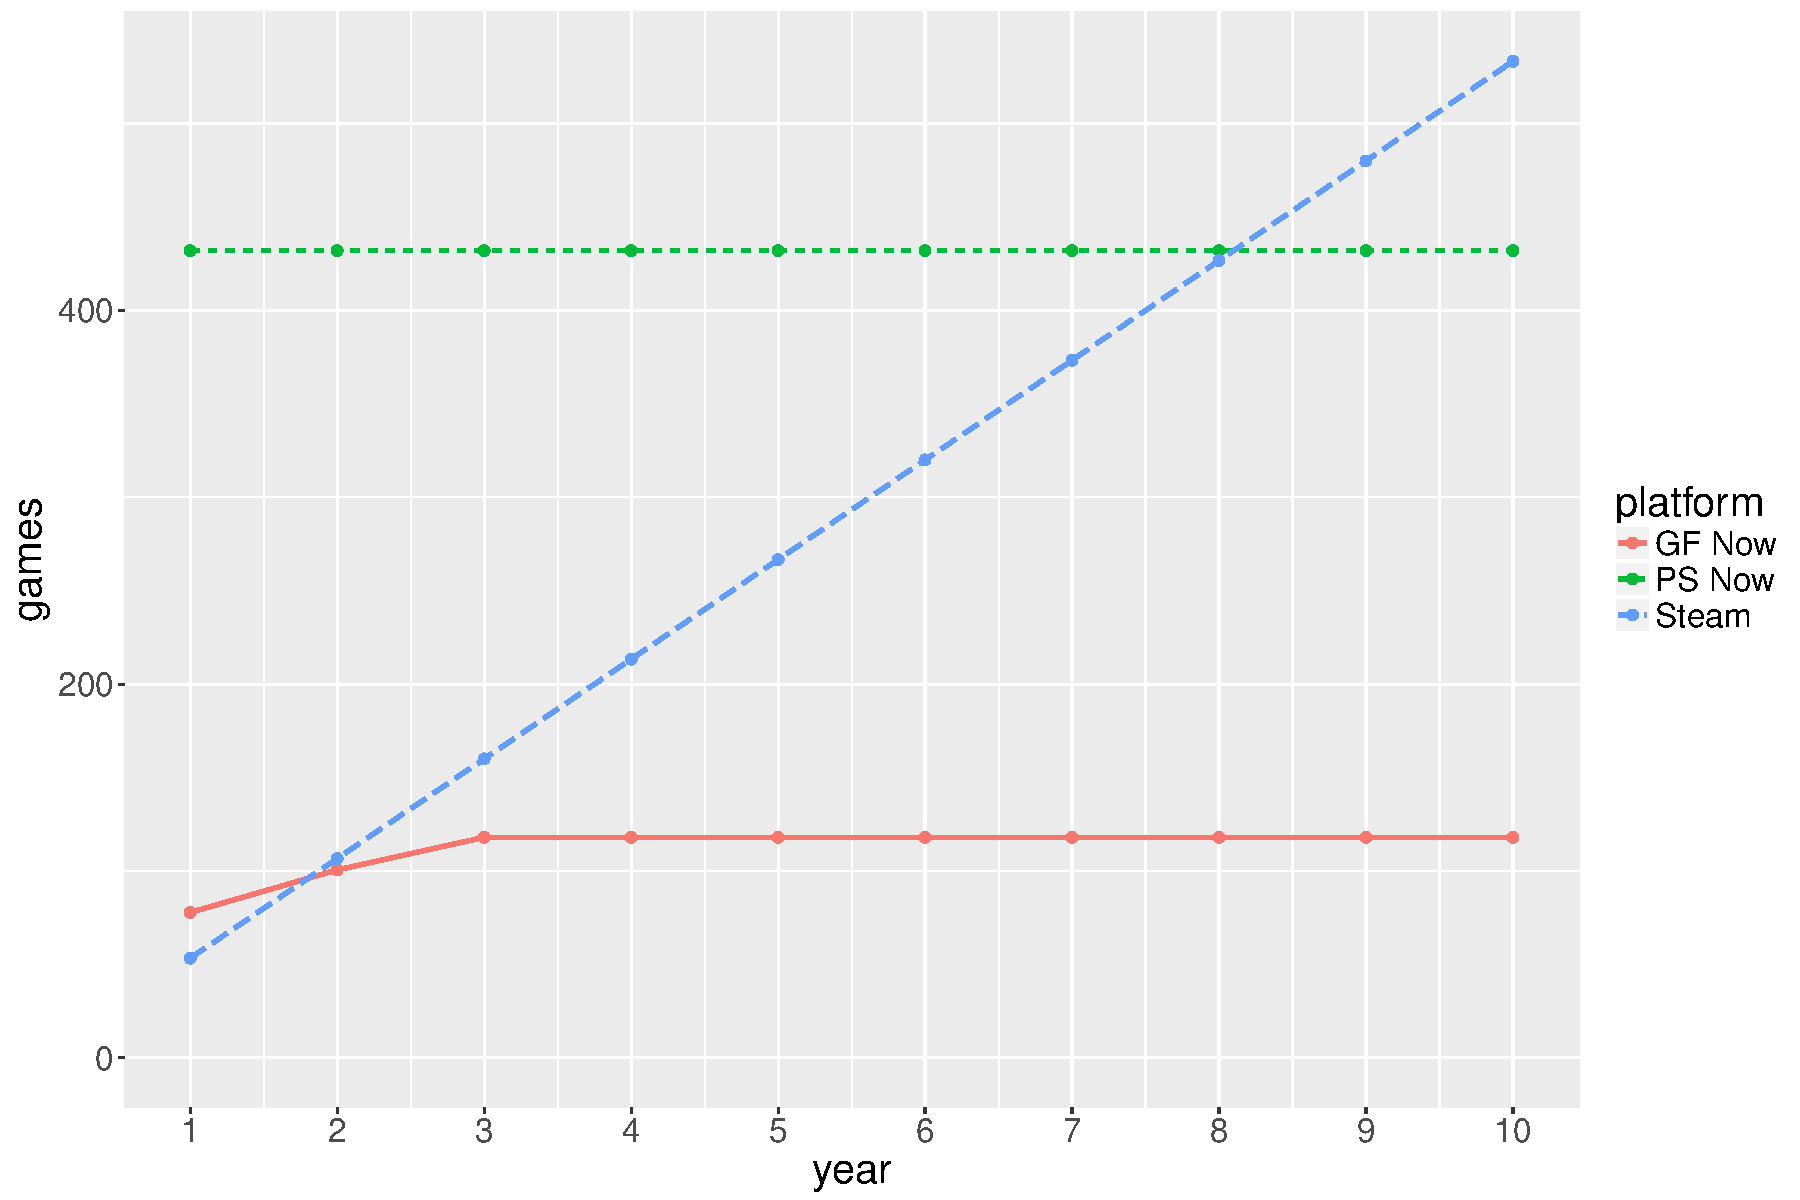
\includegraphics[width=1.0\columnwidth]{images/games-over-year.pdf}
	\caption{Number of available games per platform (y-axis) with constant customer expenditure over time (x-axis).}
\label{fig:games-over-years}
\end{figure}

Fig.~\ref{fig:games-over-years} depicts this example over ten years. The continual subscription costs limit the remaining budget for additional rental titles until the maximum number of titles is reached with that particular service, whereas the number of titles from \steam will just climb steadily. The benefits of a multi-year commitment to these Cloud Gaming services therefore seem to be very limited, especially when considering, that no games are retained after ending the subscription.


%%%%%%%%%%%%%%%%%%%%%%%%%%%%%%%%%%%%%%%%%%%%%%%%%%%%%%%%%%%%%%%%%%%%%%%%%%%%%%%%
\subsection{Discussion}

Summing this section up, the investigated simple engagement metrics somewhat expose the difference between an open market platform and the curated-by-necessity cloud gaming services. The size and sales-based price model of \steam poses challenges for direct competitors such as \gfnow. Services that cater to different audiences, such as \psnow which positions itself as a backwards compatibility service, may have more success in this regard. However, the limited target audience of \psnow becomes even narrower when the high subscription costs are taken into account, diminishing the benefits for many, not even considering the additional quality challenges that streaming video games brings along. All in all this may make curated Cloud Gaming services financially unattractive for the service's operator as is discussed in the following section.

% \todo[inline]{PZ: Ist Grafik \ref{fig:games-over-years} die Basis fuer die Steigung bei ps now usw. ab dem Eintritt in Fig.~\ref{fig:gamesperyear-over-budget}. Ps now wuerde ich als Club Good sehen.}
% \todo[inline]{FM: psnow/clubgood in the sense of a backwards compatibility service for devices that do not have native access to the streamed titles?.}

%PS Now specifically caters towards older titles and backwards compatibility, may find a niche here
% wer ist die zielgruppe?
% was ist die beste platform?
% gibt es eine mainstream platform?
% unterschiedliche ausrichtungen?





% metacritic titles:
% PC 16192
% PS4 817
% XB1 588
% WiiU 474
% 3DS 871
% GFNOW 68
% PSNOW 243
% STEAM 7749



% \begin{figure}[!t]
% 	\centering
% 	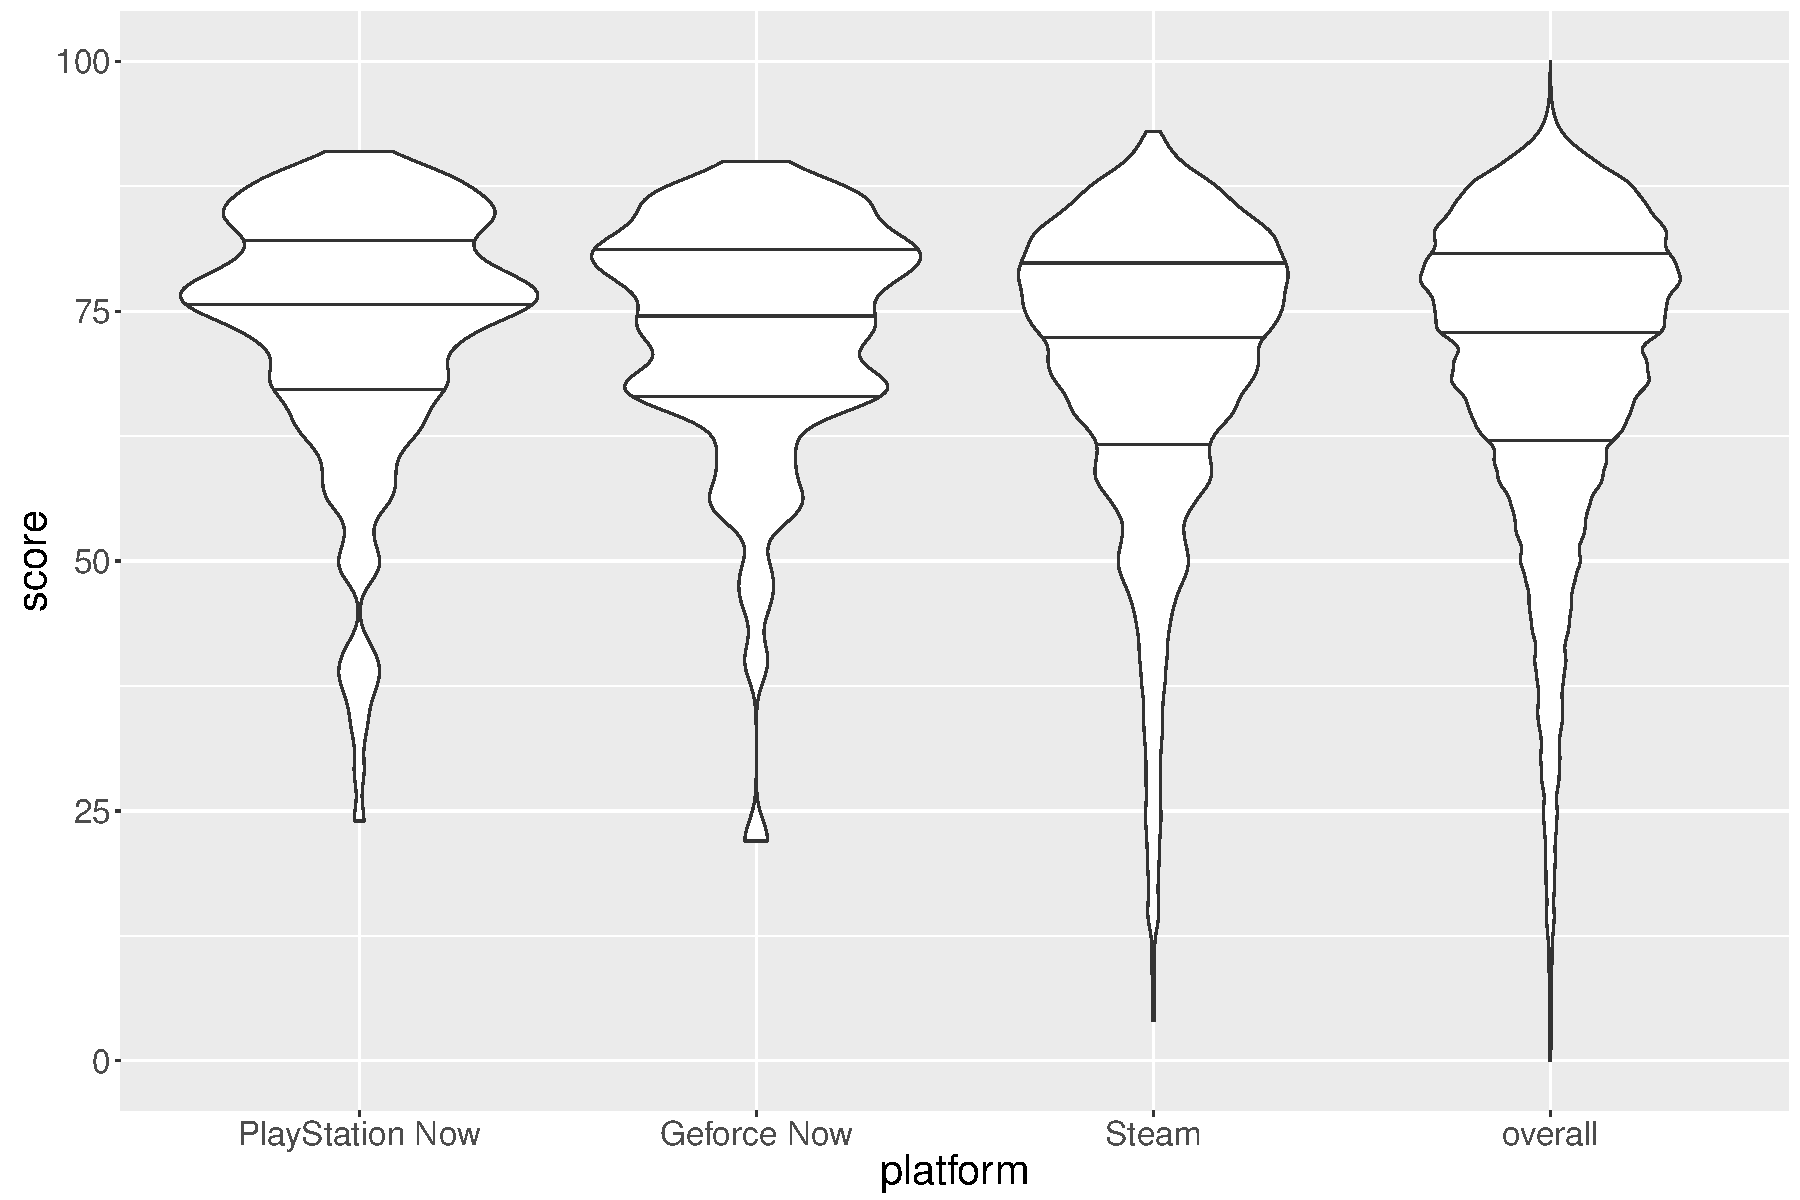
\includegraphics[width=1.0\columnwidth]{images/scores-by-platform-violin-userscore.pdf}
% 	\caption{Distribution of Metacritic user scores across the investigated platforms, depicted as violin plot with $25\%$, $50\%$, $75\%$ quantiles drawn.}
% \label{fig:userscores-by-platform}
% \end{figure}


% \subsection{E2E Lag}
% End-to-End Lag Model and Simulation in R. Now a standalone (submitted) paper at \url{https://github.com/mas-ude/onlinegame-lag-sim}. Can be referenced to argue the need for low E2E lag (meaning low network delay, but also the need for high fps).


%\item Graphical fidelity
%\item , tightness/precision/quality of controls and game mechanics, e2e lag
%\item Story?
%\item Other popularity measures? %(e.g. steamspy owner data?)
%\item Hardware requirements of games?
%\item Game costs and price history



% Caution: 
% Steam means game ownership
% PS/GF Now means only games during subscription plus permanent rental as long the sub is active(?)
% Additionally, PS Now means renting for 30 days
%!TEX root = paper.tex
%%%%%%%%%%%%%%%%%%%%%%%%%%%%%%%%%%%%%%%%%%%%%%%%%%%%%%%%%%%%%%%%%%%%%%%%%%%%%%%
%\section{Cloud Gaming Provider Models}

\section{Supply-Side Efficiency Modelling} % OR ONLY: THE SUPPLIER'S PROBLEM

%%%%%%%%%%%%%%%%%%%%%%%%%%%%%%%%%%%%%%%%%%%%%%%%%%%%%%%%%%%%%%%%%%%%%%%%%%%%%%%

%\subsection{Computational Efficiency}

Based on the collected consumer price figures of Section XXX, this section will elaborate on the required computational efficiency, i.e., cost per hosted subscriber, in order to successfully establish cloud gaming approaches on the market. Due to the limited available data, this investigation will follow a one data center assumption. Due to the demands of cloud gaming to serve both high performance and low latency, regional data centers will play a dominant role in the provider side cost modelling. Following this assumption, hereinafter a specific model is created that characterises at which cost efficiency levels the cloud gaming business can be operated successfully.

\begin{figure}[!t]
	\centering
	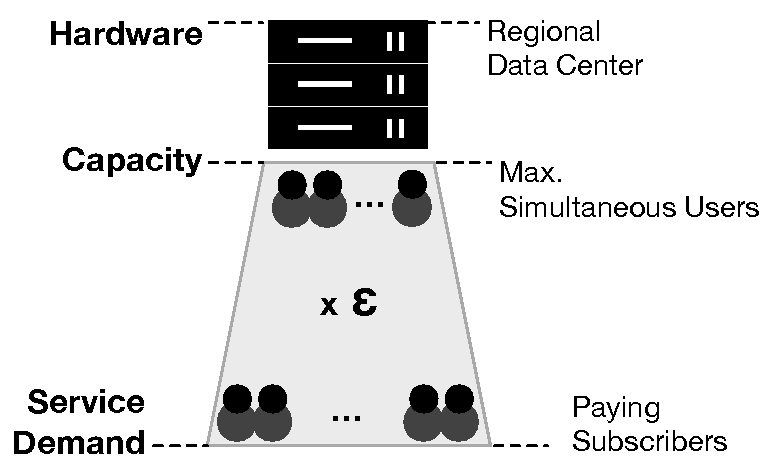
\includegraphics[width=0.65\columnwidth]{images/overbooking_datacenter.pdf}
	\caption{Overbooking of available computational capacity.}
\label{fig:overbooking_datacenter}
\end{figure}

The computational efficiency considers the maximum overbooking rate $\epsilon \geq 1$, where $\epsilon = 1$ refers to no overbooking. $\epsilon$ is calculated as ratio of the peak utilization $d_{peak}$ (number of peak time users) from the overall capacity $Cap$, 

\begin{equation}
	\epsilon = \frac{Cap}{d_{peak}} \quad ,
\end{equation}

where $Cap$ refers to the number of subscribed users that can be handled simultaneously by this data center. The maximum number of subscribers $d$ (maximum service demand) is, thus, given by

\begin{equation}
	 d = Cap \cdot \epsilon \quad .
\end{equation}

The average monthly customer price $\bar{p}$ aggregates the monthly subscription fee and the customer's depreciation costs for the hardware investments on a four years investment duration. We further consider a minimum profit margin $m$ of $3 \%$, which is in line with the average figure for the global game industry\footnote{\url{http://www.polygon.com/2012/10/1/3439738/the-state-of-games-state-of-aaa}} and substantially below the cloud computing figures that can range up to $16.9\%$\footnote{\url{http://www.forbes.com/sites/georgeanders/2015/04/23/amazons-web-services-delight-16-9-margins-more-joy-ahead/\#73324aa64b4e}} and potentially even higher\footnote{\url{http://www.bloomberg.com/news/articles/2015-12-02/microsoft-should-disclose-cloud-revenue-margins-ballmer-says}}.

%Global Games statistics / billion revenues 2012-2016: http://newzoo.com/infographics/global-games-market-report-infographics-2013/
% Game industry = 3%: http://www.polygon.com/2012/10/1/3439738/the-state-of-games-state-of-aaa
% Game industry in the past (2009 – average console game with margin of 40%): http://www.businessinsider.com/casual-gaming-profit-margins-near-90-2009-10?IR=T
% Profit margins in cloud computing:
%	Amazon 16.9% (2015): http://www.forbes.com/sites/georgeanders/2015/04/23/amazons-web-services-delight-16-9-margins-more-joy-ahead/#73324aa64b4e
% 	Microsoft 44% (2015) -- questionable: http://www.bloomberg.com/news/articles/2015-12-02/microsoft-should-disclose-cloud-revenue-margins-ballmer-says

\begin{align} \label{eq:computational_efficiency}
	\frac{\epsilon \cdot Cap \cdot \bar{p}}{Cap} :=& \underbrace{\frac{C_{cap}}{Cap}}_{C_{u}} \cdot m =\\
	= C_{u} = \frac{C_{cap}}{Cap} :=& \epsilon \cdot \bar{p}
\end{align}

When treating the costs of the regional data center as blackbox (operational and capital costs for the data center, and required game licensing fees), the analysis can concentrate on the required capacity and licensing cost $C_{u}$ per connected user $u$.

%\begin{equation}
%	ce = \frac{C_{cap}}{Cap} \quad .
%\end{equation}

%%%%%%%%%%%%%%%%%%%%%%%%%%%%%%%%%%%%%%%%%%%%%%%%%%%%%%%%%%%%
%SOME DATA CONSIDERATIONS:
%According to http://venturebeat.com/2014/01/15/steam-has-75-million-registered-users-third-party-steam-controllers-and-other-tidbits-from-valves-dev-days/
% Customer base of Steam was 75 Million active users in 2014. 
% %Vermutlich Nutzerzahl mittlerweile hoeher. Schaetzungen waeren also konservativ ausgerichtet.
%According to http://store.steampowered.com/stats/?l=german
% Höchststand (simultaneous): 12 406 722 Nutzer maximal, Feb 13 - Feb 15
% Peak immer abends. Niedrigster Wert bei <7.5 Mio Nutzern
% => \epsilon von 75/12,406722 = 6,0451100621
% Eigentlich, da steam wächst, > 6 eine gute Annahme. Wir könnten versuchen Schranken zu definieren.
% Wenn wir annehmen, dass Skalierung gut funktioniert, benoetigen wir keinen Buffer. Sollen wir Buffer verwenden?
%%%%%%%%%%%%%%%%%%%%%%%%%%%%%%%%%%%%%%%%%%%%%%%%%%%%%%%%%%%%

\todo[inline]{NOW LET'S ADD THE DATA. Check the 12.4 Mio. E.g. user older data. Introduce customer base data and reasoning above. Illustrate that epsilon will be around 6.}

For obtaining the required minimum margin $m$, the capacity and licensing cost per user $ce$ needs to be below XXXXXXXX Euro. Considering a capacity $Cap$ for 12.4 Mio active users, this refers to a total capacity cost $C_{Cap}$ of XXXXX Euro.

The overbooking ratio $\epsilon$ could also be increased by models fostering the off-peak usage, e.g., off-peak subscriptions that only allow access to the platform outside peak hours. When considering a substantial increase of the $\epsilon$ to $1.5$---the realistic maximum when considering the high peak time centricity of the gaming use case---, we obtain a substantially lowered $C_{u}$ requirement of 

\todo[inline]{ADD DATA}

Due to the requirement of using special hardware that is focused on the gaming use case, hardware sharing with other cloud applications seems unrealistic. Thus, we can characterise that the successful will have a maximum $C_{u}$ in the following bounds:

\todo[inline]{XXX}

This maximum does not consider that the operator may not be able to fully utilize the available capacity or may not hold the optimal game licenses at all times. Thus, in practice, the required hardware costs per subscriber have to be lower than $C_{u}$ .

\todo[inline]{NOW LET'S INTERPRET IF THAT SOUNDS LIKE A HARD THING TO DO OR NOT. AND THERE WE GO.}




%!TEX root = paper.tex
%%%%%%%%%%%%%%%%%%%%%%%%%%%%%%%%%%%%%%%%%%%%%%%%%%%%%%%%%%%%%%%%%%%%%%%%%%%%%%%%
\section{Conclusion}
\label{sec:conclusion}

While cloud gaming is a topic of strong interest, it comes with a series of problems and limitations, both technical as well as economic in nature. With the conducted user-side analysis it is easy to see the different, curated nature of current cloud gaming services, with their narrow offer of hand-selected games, in the case of \psnow even catered to a specific audience. This limits the attractiveness of any such service, even without looking at more intricate engagement metrics which would require more data than what was available.

But also the operator-side reveals major problems due to the need for highly regional data-centers and special hardware. This eliminates any chance for the efficiency gains that general cloud services are intended for.

However, there might be some niches for specific games or audiences that could be sustained at reduced operational efforts. This might be an angle worth of investigation in the future, especially with better engagement metrics and more detailed models of gaming data center operations.

However, there might also be a simpler and economically more feasible alternative to cloud gaming: game streaming in the local network, which would combine the open market structures of conventional gaming platforms with the ease of use of having a small box in the living that one just can play games on without much thought to the underlying hardware.


\printbibliography 

\balance

\end{document}
